\documentclass[a4paper,12pt,oneside]{book}
\usepackage{times}
\usepackage[utf8]{vietnam}
\usepackage[shortlabels]{enumitem}
\usepackage{booktabs}
\usepackage{colortbl}
\usepackage{setspace}
\usepackage{amsmath,amssymb}
\hyphenation{Journal Journals}
\usepackage[left=3cm,right=2cm,top=2.5cm,bottom=3cm,footskip=40pt]{geometry}
\usepackage{array}
\newcolumntype{C}[1]{>{\centering\let\newline\\\arraybackslash\hspace{0pt}}m{#1}}
\usepackage{tabularx}
\usepackage{multirow}
\usepackage{multicol}
\usepackage{longtable}
\setcounter{secnumdepth}{4}
\usepackage{placeins}
\usepackage{indentfirst}
\setlength{\parindent}{1cm}
\usepackage{color}
\usepackage{fancyhdr}
\usepackage{fncychap}
\usepackage{graphicx}
\usepackage{etoolbox}
\usepackage{listings}
\usepackage{xcolor}
\usepackage{tikz}
\usetikzlibrary{calc}
\usepackage{titlesec}
\usepackage[labelsep=period]{caption}
\graphicspath {{figures/}}

\DeclareCaptionFormat{myformat}{\fontsize{13}{15}\selectfont#1#2#3}
\captionsetup{format=myformat}

\titlelabel{\thetitle.\,\,}
\titleformat{\chapter}[display]
  {\fontsize{14}{16}\selectfont\bfseries\centering}
  {\MakeUppercase{\chaptertitlename}\ \thechapter}{0pt}{\fontsize{14}{16}\selectfont\MakeUppercase}
\titlespacing{\chapter}{0pt}{0pt}{40pt}
\titleformat*{\section}{\fontsize{14}{14}\selectfont\bfseries}
\titleformat*{\subsection}{\fontsize{14}{14}\selectfont\bfseries\slshape}
\titleformat*{\subsubsection}{\fontsize{14}{14}\slshape}
\titlespacing\section{0pt}{6pt plus 4pt minus 2pt}{1pt plus 2pt minus 2pt}
\titlespacing\subsection{0pt}{6pt plus 4pt minus 2pt}{1pt plus 2pt minus 2pt}
\titlespacing\subsubsection{0pt}{6pt plus 4pt minus 2pt}{0pt plus 2pt minus 2pt}

\usepackage{titletoc}
\usepackage{tocloft}
\cftsetpnumwidth{20pt}
\titlecontents{chapter}
  [0pt]
  {}
  {\fontsize{13.5}{14}\selectfont\MakeUppercase{\chaptername}\ \thecontentslabel.\,\,}
  {}
  {\cftdotfill{\cftdotsep}\contentspage}
\renewcommand{\cftsecaftersnum}{.}%
\renewcommand{\cftsubsecaftersnum}{.}%

\renewcommand{\cftfigfont}{Hình~}
\renewcommand{\cfttabfont}{Bảng~ }
\renewcommand{\lstlistingname}{Mã nguồn}

\renewcommand{\baselinestretch}{1.4}
\flushbottom

% -- Cau hinh khung code (listings) --
\definecolor{codebg}{RGB}{244,244,244}
\definecolor{codeframe}{RGB}{180,180,180}
\definecolor{codekw}{RGB}{0,0,160}
\definecolor{codecmt}{RGB}{0,128,0}
\lstset{
  basicstyle=\ttfamily\fontsize{9}{11}\selectfont,
  backgroundcolor=\color{codebg},
  frame=single, rulecolor=\color{codeframe},
  breaklines=true, breakatwhitespace=false,
  columns=fullflexible, keepspaces=true,
  showstringspaces=false,
  xleftmargin=8pt, xrightmargin=4pt, framexleftmargin=4pt,
  aboveskip=8pt, belowskip=8pt,
}
% listings khong co san ngon ngu JSON -> dinh nghia toi thieu
\lstdefinelanguage{json}{
  morestring=[b]",
  showstringspaces=false,
  comment=[l]{//},
}

\usepackage[hidelinks, unicode]{hyperref}

% Cho phep ngat dong sau dau gach duoi trong \texttt (ten bien/ham dai dai) de tranh tran le
\renewcommand{\_}{\textunderscore\allowbreak}

% Tieng Viet khong co luat ngat am tiet -> cho phep gian dong de tranh tran le van xuoi
\setlength{\emergencystretch}{3em}
\hfuzz=2pt

\begin{document}
\fontsize{13}{15.5}\selectfont

\pagestyle{empty}
\begin{titlepage}
    \centering
\begin{tikzpicture}[overlay,remember picture]
\centering
\draw[line width = 3pt] ($(current page.north west) + (1.215in,-0.7in)$) rectangle ($(current page.south east) + (-0.7in,0.7in)$);
\draw (0,-24.5) node[above]{\fontsize{12}{12}\selectfont{\textbf{HÀ NỘI - 2026}}};
\end{tikzpicture}
\vspace{-1cm}
\begin{center}
\MakeUppercase{\textbf{\fontsize{12}{12}\selectfont{Đại học quốc gia hà nội}}}

\noindent{\textbf {\MakeUppercase{\fontsize{12}{12}\selectfont {trường đại học công nghệ}}}}\\
	\vspace{-0.5cm}
\vspace{2cm}
\begin{figure} [!htb]
	\centering
	
\includegraphics[width=0.2\linewidth]{figures/UET_logo.jpg}
	\label{fig:uetlogo}
\end{figure}
\vspace{1.5cm}

	{\textbf {\fontsize{14}{14}\selectfont{Nguyễn Quế Sơn}}}\\[4pt]
	{\textbf {\fontsize{14}{14}\selectfont{Nguyễn Hải An}}}\\
	\vspace{2cm}
{
{\textbf {\MakeUppercase{\fontsize{17}{18}\selectfont{Tấn công giải ẩn danh trên dữ liệu thưa}}}}\\[8pt]
{\textbf {\itshape\fontsize{13}{15}\selectfont{(Mô phỏng tấn công Netflix Prize bằng thuật toán Scoreboard-RH trên dữ liệu MovieLens)}}}\\[3pt]
}
\vspace{3cm}
\MakeUppercase{\textbf{\fontsize{14}{14}\selectfont{{Báo cáo bài tập lớn cuối kỳ}}}}\\[3pt]
{\fontsize{14}{14}\textbf{\selectfont{Học phần: An ninh di động}}}
\end{center}


\end{titlepage}

\newpage
\pagestyle{plain}
\pagenumbering{gobble}
%\addcontentsline{toc}{chapter}{Trang phụ bìa}

\begin{center}
	\begin{tikzpicture}[overlay,remember picture]
\draw[line width = 3pt] ($(current page.north west) + (1.2in,-0.7in)$) rectangle ($(current page.south east) + (-0.7in,0.7in)$);
\draw (0,-24.2) node[above]{\fontsize{12}{12}\selectfont{\textbf{HÀ NỘI - 2026}}};
\end{tikzpicture}
\end{center}
\vspace{-1.5cm}
	\begin{center}
{\MakeUppercase{\textbf{\fontsize{12}{12}\selectfont{Đại học quốc gia hà nội}}}}

\noindent\textbf {\MakeUppercase{\fontsize{12}{12}\selectfont{trường đại học công nghệ}}}\\
	\vspace{-0.5cm}
\vspace{4cm}

	{\textbf {\fontsize{14}{14}\selectfont{Nguyễn Quế Sơn}}}\\[4pt]
	{\textbf {\fontsize{14}{14}\selectfont{Nguyễn Hải An}}}\\
	\vspace{1.5cm}

{\textbf {\MakeUppercase{\fontsize{17}{18}\selectfont{Tấn công giải ẩn danh trên dữ liệu thưa}}}}\\[8pt]
{\textbf {\itshape\fontsize{13}{15}\selectfont{(Mô phỏng tấn công Netflix Prize bằng thuật toán Scoreboard-RH trên dữ liệu MovieLens)}}}\\[3pt]

\vspace{3cm}
\MakeUppercase{\textbf{\fontsize{14}{14}\selectfont{{Báo cáo bài tập lớn cuối kỳ}}}}\\[3pt]
{\fontsize{14}{14}\textbf{\selectfont{Học phần: An ninh di động}}}

\end{center}
\vspace{1.5cm}
		\begin{tabularx}
				{\linewidth}{>{\setlength\hsize{.0\hsize}}X>{\setlength\hsize{0.8\hsize}}X}
										& \fontsize{14}{14}\textbf{\selectfont{Giảng viên hướng dẫn: Lê Thị Hợi}}
	\end{tabularx}

\newpage
\def\baselinestretch{1.3}
\pagestyle{plain}
\pagenumbering{gobble}
\clearpage
\phantomsection
\addcontentsline{toc}{chapter}{Lời cam đoan}
\chapter*{Lời cam đoan}

Chúng em xin cam đoan báo cáo bài tập lớn \textit{``Tấn công giải ẩn danh trên dữ liệu thưa''} là do chúng em tự tìm hiểu, nghiên cứu và thực hiện dựa trên công trình khoa học gốc của Narayanan và Shmatikov. Toàn bộ kết quả thực nghiệm trình bày trong báo cáo là kết quả thật, thu được trực tiếp từ việc chạy ứng dụng mô phỏng do chúng em xây dựng trên tập dữ liệu công khai MovieLens 100k. Mọi thực nghiệm chỉ thao tác trên dữ liệu công khai phục vụ mục đích học thuật, không nhằm vào bất kỳ cá nhân hay hệ thống thật nào. Các tài liệu tham khảo đều đã được liệt kê đầy đủ ở phần Tài liệu tham khảo. Chúng em xin hoàn toàn chịu trách nhiệm về tính trung thực và chính xác của toàn bộ nội dung trong báo cáo này.

\vspace{1cm}

\hspace*{8.2cm}\begin{minipage}{6cm}
\centering
\textbf{Nhóm tác giả}\\[2.5cm]
\textbf{Nguyễn Quế Sơn}\\[6pt]
\textbf{Nguyễn Hải An}
\end{minipage}

\newpage
\clearpage
\phantomsection
\addcontentsline{toc}{chapter}{Lời cảm ơn}
\chapter*{Lời cảm ơn}

Chúng em xin gửi lời cảm ơn chân thành đến cô Lê Thị Hợi, giảng viên học phần An ninh di động, đã hướng dẫn, định hướng và cung cấp kiến thức nền tảng giúp chúng em hoàn thành báo cáo bài tập lớn này. Chúng em cũng xin cảm ơn các thầy cô Khoa Công nghệ thông tin, Trường Đại học Công nghệ - Đại học Quốc gia Hà Nội vì những kiến thức quý báu đã truyền đạt trong suốt quá trình học tập.

\vspace{0.3cm}

Do thời gian và kiến thức còn hạn chế, báo cáo không tránh khỏi những thiếu sót. Chúng em rất mong nhận được các góp ý của cô để hoàn thiện hơn.

\newpage

\pagenumbering{roman}

\setlength{\parindent}{1cm}
\setlength{\parskip}{0.6ex}

\fontsize{13}{16}\selectfont
\renewcommand{\contentsname}{\vspace{-70pt}\centerline{\fontsize{14}{16}\selectfont\MakeUppercase{Mục lục}}}
\clearpage
\phantomsection
\addcontentsline{toc}{chapter}{Mục lục}
\tableofcontents
\clearpage
\clearpage
\phantomsection
\addcontentsline{toc}{chapter}{Tóm tắt}
\chapter*{Tóm tắt}

\noindent\textbf{Tóm tắt:}
Báo cáo nghiên cứu và mô phỏng lại lớp tấn công giải ẩn danh (de-anonymization) trên các tập dữ liệu thưa, dựa trên công trình kinh điển \textit{``Robust De-anonymization of Large Sparse Datasets''} của Narayanan và Shmatikov - cũng chính là cuộc tấn công đã phá vỡ tính ẩn danh của tập dữ liệu Netflix Prize. Chúng em phân tích mô hình hình thức của bài toán (độ thưa, độ tương tự, định nghĩa rò rỉ riêng tư), thuật toán Scoreboard-RH cùng tiêu chí \textit{eccentricity}, sau đó xây dựng một ứng dụng web hoàn chỉnh (FastAPI + React) mô phỏng kẻ tấn công trên tập dữ liệu công khai MovieLens 100k.

Bằng thực nghiệm thật trên 943 người dùng và 100.000 lượt đánh giá, chúng em chứng minh: chỉ với 8 bộ phim + ngày xem, thuật toán định danh đúng 98\% người dùng; ngay cả khi không có thông tin ngày vẫn đạt 93\%; và với thông tin nhiễu ($\pm 1$ điểm, $\pm 14$ ngày) vẫn đạt 72\% - khẳng định tính \textit{bền vững} của tấn công. Khi ưu tiên các bộ phim hiếm, chỉ 2 phim đã đủ định danh 59\% người dùng. Báo cáo cũng so sánh, tối ưu và nâng cấp ứng dụng demo cho đúng công thức trong bài báo gốc, rồi thảo luận các biện pháp phòng vệ (k-anonymity, riêng tư vi phân, hạn chế công bố micro-data).

\vspace{0.5cm}
\noindent\textit{\textbf{Từ khóa:}} \textit{giải ẩn danh, dữ liệu thưa, quyền riêng tư, Netflix Prize, MovieLens, Scoreboard-RH, eccentricity.}

\newpage
\clearpage
\phantomsection
\addcontentsline{toc}{chapter}{Danh sách từ viết tắt}
\chapter*{Danh sách từ viết tắt}

\renewcommand{\arraystretch}{1.3}
\noindent
\begin{tabularx}{\linewidth}{p{2.8cm} X}
\textbf{Từ viết tắt} & \textbf{Giải nghĩa} \\[2pt]
PII & Personally Identifiable Information - Thông tin định danh cá nhân \\
aux & Auxiliary information - Tri thức bổ trợ kẻ tấn công nắm giữ \\
supp & Support - Tập thuộc tính khác rỗng của một bản ghi / số người đánh giá một phim \\
RH & Robust, Histogram - Biến thể bền vững của thuật toán Scoreboard \\
ecc & Eccentricity - Độ ``nổi bật'' của ứng viên khớp nhất so với phần còn lại \\
DP & Differential Privacy - Riêng tư vi phân \\
API & Application Programming Interface \\
REST & Representational State Transfer \\
CSV & Comma-Separated Values \\
ORM & Object-Relational Mapping \\
UI & User Interface - Giao diện người dùng \\
\end{tabularx}

\newpage

\clearpage
\phantomsection
\addcontentsline{toc}{chapter}{Danh mục hình vẽ}
\renewcommand{\listfigurename}{\vspace{-70pt}\centerline{\fontsize{14}{16}\selectfont{\MakeUppercase{Danh mục hình vẽ}}}}
\listoffigures
\fontsize{13}{16}\selectfont
\newpage

\clearpage
\phantomsection
\addcontentsline{toc}{chapter}{Danh mục bảng biểu}
\renewcommand{\listtablename}{\vspace{-70pt}\centerline{\fontsize{14}{16}\selectfont{\MakeUppercase{Danh mục bảng biểu}}}}
\listoftables
\fontsize{13}{16}\selectfont
\newpage

\pagenumbering{arabic}
\pagestyle{plain}

\clearpage
\phantomsection
\addcontentsline{toc}{chapter}{Mở đầu}
\chapter*{Mở đầu}

\section*{Bối cảnh và động lực}
Ngày nay, các tổ chức thường xuyên công bố những tập dữ liệu lớn về hành vi cá nhân - lịch sử mua hàng, đánh giá phim, lượt nghe nhạc, vị trí di chuyển - phục vụ nghiên cứu, khuyến nghị và khai phá dữ liệu. Để bảo vệ người dùng, các đơn vị này thường ``ẩn danh hóa'' dữ liệu bằng cách loại bỏ tên, số định danh và các thông tin nhận dạng trực tiếp. Một quan niệm phổ biến cho rằng: chỉ cần gỡ bỏ thông tin định danh là dữ liệu đã an toàn.

Năm 2008, Arvind Narayanan và Vitaly Shmatikov đã bác bỏ quan niệm đó. Trong công trình \textit{``Robust De-anonymization of Large Sparse Datasets''}~\cite{narayanan}, hai tác giả chứng minh rằng với một tập dữ liệu thưa và nhiều chiều (như lịch sử xem phim), kẻ tấn công chỉ cần biết một vài thông tin bên lề về nạn nhân là đủ để xác định chính xác bản ghi của người đó và phơi bày toàn bộ phần dữ liệu còn lại. Họ áp dụng phương pháp này lên tập dữ liệu Netflix Prize - gồm hơn 100 triệu lượt đánh giá phim của 500.000 thuê bao - và định danh thành công nhiều cá nhân, làm lộ cả những thông tin nhạy cảm như xu hướng chính trị hay sở thích cá nhân. Kết quả này về sau dẫn tới một vụ kiện và khiến Netflix hủy bỏ cuộc thi Netflix Prize lần thứ hai.

Đây là một trong những minh chứng nền tảng cho thấy ``ẩn danh hóa'' không đồng nghĩa với ``riêng tư'', và là bài học cốt lõi trong lĩnh vực an toàn dữ liệu nói chung cũng như an ninh trên thiết bị, ứng dụng di động nói riêng - nơi dữ liệu hành vi người dùng được thu thập với mật độ dày đặc.

\section*{Mục tiêu}
Báo cáo đặt ra các mục tiêu sau:
\renewcommand{\labelitemi}{$-$}
\begin{itemize}
	\item Nghiên cứu và trình bày lại mô hình tấn công giải ẩn danh của Narayanan-Shmatikov: nền tảng lý thuyết (độ thưa, độ tương tự, định nghĩa rò rỉ riêng tư) và thuật toán Scoreboard-RH.
	\item Xây dựng, tối ưu và nâng cấp một ứng dụng web mô phỏng cuộc tấn công trên tập dữ liệu công khai MovieLens 100k, đóng vai proxy cho tập Netflix.
	\item Thực nghiệm định lượng thật để kiểm chứng các kết luận của bài báo gốc: cần bao nhiêu tri thức bổ trợ để định danh thành công, và mức độ bền vững của tấn công trước thông tin sai lệch.
	\item Thảo luận ý nghĩa về quyền riêng tư và các biện pháp phòng vệ.
\end{itemize}

\section*{Phạm vi và phương pháp}
Toàn bộ thực nghiệm chỉ thao tác trên tập dữ liệu công khai MovieLens 100k, trong môi trường cục bộ, không nhằm vào bất kỳ cá nhân hay hệ thống thật nào. Mọi số liệu, biểu đồ và ảnh chụp màn hình trong báo cáo đều là kết quả thật, sinh ra trực tiếp từ việc chạy ứng dụng do chúng em phát triển. Ngôn ngữ cài đặt là Python (engine tấn công, FastAPI) và JavaScript/React (giao diện).

\section*{Cấu trúc báo cáo}
Chương~\ref{chap:background} trình bày cơ sở lý thuyết về bài toán giải ẩn danh và thuật toán Scoreboard-RH. Chương~\ref{chap:design} phân tích bài toán và thiết kế kiến trúc hệ thống mô phỏng. Chương~\ref{chap:impl} mô tả chi tiết việc cài đặt thuật toán cùng những tối ưu, nâng cấp so với bản demo ban đầu. Chương~\ref{chap:exp} trình bày kịch bản demo và các kết quả thực nghiệm định lượng. Chương~\ref{chap:conclusion} thảo luận biện pháp phòng vệ, nêu hạn chế và kết luận.

\newpage
\chapter{Cơ sở lý thuyết}
\label{chap:background}

Chương này trình bày nền tảng lý thuyết của tấn công giải ẩn danh: từ hạn chế của các phương pháp ẩn danh truyền thống, mô hình hình thức hóa bài toán, thuật toán Scoreboard-RH và phân tích lý thuyết về lượng tri thức cần thiết, đến tình huống điển hình Netflix Prize và mối liên hệ với an ninh di động. Nội dung chương dựa chủ yếu trên công trình gốc của Narayanan và Shmatikov~\cite{narayanan}, có bổ sung từ các công trình liên quan.

\section{Bài toán ẩn danh hóa micro-data}

\textit{Micro-data} là dữ liệu ở mức từng cá nhân: mỗi bản ghi mô tả một người và gồm nhiều thuộc tính. Khác với dữ liệu thống kê tổng hợp (chỉ công bố các đại lượng gộp như trung bình, tổng), micro-data giữ lại bản ghi riêng của từng người ngay cả sau khi đã ``ẩn danh hóa''. Các tập như lịch sử mua hàng, hồ sơ y tế, log tìm kiếm, dấu vết di chuyển GPS hay lịch sử xem phim đều là micro-data.

Nhu cầu công bố micro-data ngày càng lớn: phục vụ nghiên cứu y học, huấn luyện hệ khuyến nghị, minh bạch hóa dữ liệu công (``open data''). Để bảo vệ người dùng, đơn vị công bố thường \textit{loại bỏ thông tin định danh trực tiếp} (Personally Identifiable Information - PII) như họ tên, số căn cước, địa chỉ. Câu hỏi trung tâm của chương này là: \textit{liệu việc gỡ bỏ PII có thực sự bảo vệ được quyền riêng tư hay không?}

Câu trả lời là không. Hai đặc trưng của micro-data hành vi - \textit{số chiều cao} (high dimensionality) và \textit{độ thưa} (sparsity) - khiến mỗi bản ghi gần như là một ``dấu vân tay'' duy nhất, có thể bị liên kết ngược về danh tính thật chỉ với một lượng nhỏ thông tin bên lề.

\section{Các phương pháp ẩn danh truyền thống và hạn chế}

\subsection{k-anonymity}
Mô hình bảo vệ kinh điển nhất là k-anonymity~\cite{sweeney}. Đơn vị công bố chia thuộc tính thành hai nhóm:
\renewcommand{\labelitemi}{$-$}
\begin{itemize}
	\item \textit{Quasi-identifier} (QID): các thuộc tính tuy không định danh trực tiếp nhưng có thể liên kết với nguồn dữ liệu khác để truy ra danh tính (ví dụ: tuổi, giới tính, mã vùng bưu chính).
	\item \textit{Thuộc tính nhạy cảm}: thông tin cần bảo vệ (ví dụ: bệnh án, mức lương).
\end{itemize}
Dữ liệu được \textit{khái quát hóa} (generalization) và \textit{nén} (suppression) sao cho mỗi tổ hợp giá trị QID xuất hiện ở ít nhất $k$ bản ghi. Như vậy, một bản ghi không thể bị phân biệt khỏi $k-1$ bản ghi khác cùng nhóm QID.

Động lực của k-anonymity đến từ một vụ tấn công thực tế: năm 1997, L. Sweeney liên kết tập dữ liệu xuất viện ``ẩn danh'' của bang Massachusetts (gồm mã vùng, ngày sinh, giới tính) với danh sách cử tri công khai, và truy ra được \textit{bệnh án của chính thống đốc bang}~\cite{sweeney}. Chỉ ba thuộc tính tưởng như vô hại đã đủ định danh phần lớn dân số Hoa Kỳ.

\subsection{l-diversity, t-closeness và giới hạn chung}
k-anonymity bảo vệ khỏi việc \textit{định danh bản ghi}, nhưng không bảo vệ giá trị nhạy cảm. Nếu cả $k$ bản ghi trong một nhóm QID đều có cùng giá trị nhạy cảm (tấn công đồng nhất - homogeneity attack), kẻ tấn công vẫn suy ra được giá trị đó. Các cải tiến ra đời để vá lỗ hổng này:
\begin{itemize}
	\item \textbf{l-diversity}~\cite{ldiversity}: yêu cầu mỗi nhóm QID chứa ít nhất $l$ giá trị nhạy cảm ``đủ khác biệt''.
	\item \textbf{t-closeness}~\cite{tcloseness}: yêu cầu phân phối thuộc tính nhạy cảm trong mỗi nhóm gần với phân phối toàn cục (khoảng cách $\le t$).
\end{itemize}

Tuy nhiên, toàn bộ họ phương pháp này có một giả định nền tảng bị phá vỡ khi áp dụng cho micro-data hành vi: chúng giả định có thể \textit{tách trước} tập QID khỏi thuộc tính nhạy cảm. Với dữ liệu như lịch sử xem phim, giả định này sai về bản chất:
\renewcommand{\labelitemi}{$-$}
\begin{itemize}
	\item \textbf{Mọi thuộc tính đều có thể là QID.} Kẻ tấn công có thể biết \textit{bất kỳ} bộ phim nào về nạn nhân; không thể chỉ định trước một tập QID cố định.
	\item \textbf{Thất bại trên dữ liệu nhiều chiều.} Khi số thuộc tính lên tới hàng nghìn, để mọi tổ hợp xuất hiện $\ge k$ lần phải khái quát hóa mạnh tới mức dữ liệu mất hết giá trị sử dụng~\cite{narayanan}.
\end{itemize}
Chính vì vậy, tập Netflix Prize - như sẽ thấy - hoàn toàn \textit{không} $k$-ẩn danh với bất kỳ $k > 1$ nào.

\subsection{Các tiền lệ rò rỉ thực tế}
Ngoài vụ Massachusetts, hai vụ việc nổi tiếng khác minh họa rủi ro:
\begin{itemize}
	\item \textbf{AOL (2006):} AOL công bố 20 triệu truy vấn tìm kiếm ``ẩn danh'' (chỉ thay tên người dùng bằng số). Phóng viên New York Times đã truy ra danh tính người dùng số 4417749 chỉ từ nội dung các truy vấn của bà~\cite{aol}.
	\item \textbf{MovieLens (2006):} Frankowski và cộng sự liên kết các bài đăng công khai trên diễn đàn MovieLens với hồ sơ đánh giá nội bộ, cho thấy ngay cả ``đề cập công khai'' về phim cũng đủ gây rò rỉ~\cite{frankowski}.
\end{itemize}

\section{Độ thưa và độ tương tự}

Quan sát then chốt của Narayanan-Shmatikov là các tập dữ liệu hành vi thực tế đều thưa: mỗi người chỉ tương tác với một phần rất nhỏ trong không gian thuộc tính khổng lồ. Trên tập Netflix, mỗi thuê bao chỉ đánh giá vài chục đến vài trăm phim trong số hàng chục nghìn phim. Hệ quả là mỗi bản ghi gần như duy nhất: rất khó tìm được hai người có cùng tổ hợp phim và điểm. Chính sự duy nhất này là mầm mống của rò rỉ riêng tư.

Gọi $\mathrm{supp}(r)$ là \textit{support} của bản ghi $r$ - tập các thuộc tính khác rỗng (các phim mà người đó đã đánh giá). Phân phối số người đánh giá mỗi phim tuân theo quy luật ``đuôi dài'' (long-tail) hay luật lũy thừa: một số ít phim bom tấn được rất nhiều người xem, còn phần lớn phim chỉ có ít người xem. Các phim hiếm ở phần đuôi mang giá trị định danh cao.

Để đo mức ``giống nhau'' giữa hai bản ghi, ta dùng hàm tương tự $\mathrm{Sim}(r_1, r_2) \in [0,1]$. Một cách hình thức, bài báo định nghĩa tính thưa như sau:

\vspace{0.2cm}
\noindent\textbf{Định nghĩa (Độ thưa).} \textit{Một cơ sở dữ liệu $D$ được gọi là $(\epsilon, \delta)$-thưa theo độ tương tự $\mathrm{Sim}$ nếu}
\begin{equation}
	\Pr_{r}\big[\, \exists\, r' \neq r : \mathrm{Sim}(r, r') > \epsilon \,\big] \le \delta
\end{equation}
\textit{nghĩa là xác suất một bản ghi ngẫu nhiên có ``hàng xóm gần'' với độ tương tự vượt $\epsilon$ là không quá $\delta$.}\footnote{Bài báo gốc viết điều kiện trong ngoặc dưới dạng $\mathrm{Sim}(r,r')>\epsilon\ \forall r'\neq r$. Ở đây chúng em dùng lượng từ $\exists$ cho đúng với ngữ nghĩa mà chính bài báo mô tả - ``không tồn tại bản ghi nào khác đủ giống'' - tức xác suất một bản ghi có ít nhất một hàng xóm gần là rất nhỏ.}

\vspace{0.2cm}
Bài báo chứng minh tập Netflix thưa áp đảo: với đại đa số bản ghi, không tồn tại bản ghi nào khác có độ tương tự trên $0{,}5$ trong toàn bộ 500.000 bản ghi - ngay cả khi chỉ xét tập phim đã xem mà bỏ qua điểm số và ngày.

\section{Mô hình tấn công và định nghĩa rò rỉ riêng tư}

\subsection{Tri thức bổ trợ}
Kẻ tấn công có một tập \textit{aux} $= \mathrm{Aux}(r)$ - thông tin bên lề về nạn nhân $r$, gồm giá trị của một tập con nhỏ các thuộc tính. Điểm mấu chốt làm nên tên gọi ``robust'': aux không cần chính xác - điểm có thể sai lệch, ngày có thể chỉ biết gần đúng, thậm chí một vài mục hoàn toàn sai. Một cách hình thức, $\mathrm{Aux}$ được mô hình hóa như một hàm xác suất ánh xạ bản ghi thật sang phiên bản nhiễu mà kẻ tấn công nắm giữ. Kẻ tấn công có thể thu thập aux từ trò chuyện đời thường, mạng xã hội, hay đánh giá công khai của nạn nhân trên một dịch vụ khác.

\subsection{Hai kịch bản rò rỉ}
Bài báo phân biệt hai dạng vi phạm riêng tư:
\renewcommand{\labelitemi}{$-$}
\begin{itemize}
	\item \textbf{Giải ẩn danh ``đoán tốt nhất'' (best-guess):} thuật toán đưa ra \textit{một} bản ghi $r'$ và khẳng định đó là nạn nhân. Vi phạm xảy ra nếu $\mathrm{Sim}(r, r') \ge \theta$ với xác suất cao.
	\item \textbf{Giải ẩn danh ``danh sách nghi phạm'' (lineup):} thuật toán đưa ra một tập nhỏ ứng viên kèm phân phối xác suất, tương tự khái niệm ẩn danh trong mạng trộn (mix network). Mức rò rỉ được đo bằng \textit{entropy} của phân phối: kẻ tấn công cần thêm bao nhiêu bit thông tin để xác định duy nhất nạn nhân.
\end{itemize}
Vì dữ liệu thưa, bản ghi thỏa $\mathrm{Sim}(r, r') \ge \theta$ gần như chắc chắn là duy nhất - nên danh sách nghi phạm thường thu về đúng một người. Khi đó kẻ tấn công học được \textit{toàn bộ} thuộc tính của bản ghi đó, kể cả các thuộc tính nhạy cảm mà ban đầu hắn không biết.

\section{Thuật toán Scoreboard và Scoreboard-RH}

Thuật toán giải ẩn danh được mô tả như một \textit{khuôn mẫu} (template) gồm ba thành phần:
\begin{enumerate}[1.]
	\item \textbf{Hàm cho điểm} $\mathrm{Score}(aux, r')$: gán cho mỗi bản ghi ứng viên một điểm thể hiện mức khớp với aux.
	\item \textbf{Tiêu chí khớp} (matching): từ tập điểm, quyết định có một khớp hay không.
	\item \textbf{Chọn bản ghi} (selection): trả về bản ghi ``đoán tốt nhất'' hoặc phân phối xác suất.
\end{enumerate}

Thuật toán cơ sở Scoreboard gán điểm bằng độ tương tự nhỏ nhất giữa ứng viên và aux, rồi chọn nếu điểm vượt một hằng số $\alpha$. Cách này không bền vững: chỉ cần một thuộc tính trong aux hoàn toàn sai là điểm sụp đổ.

Phiên bản bền vững Scoreboard-RH (Robust, Histogram) cải tiến hàm cho điểm theo hai heuristic quan trọng:

\subsection{Trọng số theo độ hiếm}
Các thuộc tính hiếm được gán trọng số lớn hơn. Biết nạn nhân xem một bộ phim nghệ thuật ít người biết có giá trị định danh cao hơn nhiều so với biết họ xem một bom tấn. Trọng số định nghĩa:
\begin{equation}
	wt(i) = \frac{1}{\log |\mathrm{supp}(i)|}
	\label{eq:weight}
\end{equation}
với $|\mathrm{supp}(i)|$ là số người đã đánh giá phim $i$. Phim càng ít người xem, $wt(i)$ càng lớn.

\subsection{Cộng gộp tương tự rating và thời gian}
Với mỗi phim $i$ trong aux, điểm tích lũy theo cả độ lệch điểm số và độ lệch thời gian, dùng hàm mũ suy giảm:
\begin{equation}
	\mathrm{Score}(aux, r') = \sum_{i \in \mathrm{supp}(aux)} wt(i)\left( e^{-\frac{|\rho_i - \rho'_i|}{\rho_0}} + e^{-\frac{|d_i - d'_i|}{d_0}} \right)
	\label{eq:score}
\end{equation}
trong đó $\rho_i, d_i$ là điểm và thời điểm trong aux; $\rho'_i, d'_i$ là của ứng viên $r'$; $\rho_0, d_0$ là hằng số co giãn (bài báo chọn $\rho_0 = 1{,}5$ và $d_0 = 30$ ngày). Hàm mũ khiến các khớp ``gần đúng'' vẫn được tính điểm dương - đây là chìa khóa của tính bền vững: một phim vẫn đóng góp ngay cả khi ngày xem sai lệch nhiều.

\subsection{Tiêu chí eccentricity}
Để quyết định ứng viên điểm cao nhất có thực sự là nạn nhân hay chỉ là trùng hợp, thuật toán dùng eccentricity: khoảng cách giữa điểm cao nhất và điểm cao nhì, chuẩn hóa theo độ lệch chuẩn của toàn bộ phân phối điểm:
\begin{equation}
	\mathrm{ecc} = \frac{\max_1 - \max_2}{\sigma}
	\label{eq:ecc}
\end{equation}
Nếu $\mathrm{ecc} > \phi$ (ngưỡng, bài báo chọn $\phi = 1{,}5$) thì ứng viên cao nhất ``nổi bật'' hẳn so với đám đông và được kết luận là nạn nhân; ngược lại, thuật toán \textit{từ chối định danh} để tránh dương tính giả. Đây là cơ chế tự kiểm soát sai số quan trọng: nó cho phép thuật toán \textit{biết khi nào nó không biết}, nhờ đó mỗi lần khẳng định đều có độ tin cậy cao.

\section{Phân tích: cần bao nhiêu tri thức bổ trợ?}

Một đóng góp lý thuyết quan trọng của bài báo là định lượng tri thức bổ trợ tối thiểu để tấn công thành công. Kết quả chính có thể phát biểu trực giác như sau: với một cơ sở dữ liệu $N$ bản ghi đủ thưa, kẻ tấn công chỉ cần biết khoảng
\begin{equation}
	m \ \ge\ \frac{\log N}{-\log(1 - \epsilon)}
\end{equation}
thuộc tính của nạn nhân (mỗi thuộc tính khớp tới độ chính xác $1-\epsilon$) là đủ để định danh duy nhất bản ghi với xác suất cao. Điều đáng chú ý là $m$ chỉ tăng theo logarit của kích thước cơ sở dữ liệu: dù dữ liệu lớn gấp nghìn lần, lượng tri thức cần thiết hầu như không đổi. Với dữ liệu \textit{thưa}, $m$ còn nhỏ hơn nữa - đây là lý do chỉ cần 5-8 thuộc tính là đủ để giải ẩn danh hầu hết bản ghi trong các tập thực tế.

Bài báo cũng chứng minh tính bền vững một cách hình thức: ngay cả khi dữ liệu công bố đã bị thêm nhiễu (sanitization) và một phần aux bị sai, thuật toán vẫn không tạo ra khớp giả với xác suất cao, miễn là dữ liệu đủ thưa. Trực giác là nhiễu nhẹ không thể ``xóa nhòa'' tính duy nhất vốn rất mạnh của các bản ghi thưa.

\section{Tình huống điển hình: tập Netflix Prize}

Năm 2006, Netflix công bố tập dữ liệu gồm hơn 100 triệu lượt đánh giá của khoảng 500.000 thuê bao (đã loại bỏ thông tin định danh) để tổ chức cuộc thi trị giá 1 triệu USD cải tiến hệ khuyến nghị. Netflix khẳng định dữ liệu an toàn vì ``mọi thông tin định danh đã được gỡ bỏ''. Tập công bố thực chất chỉ là một mẫu nhỏ (dưới $1/10$) của cơ sở dữ liệu gốc.

\subsection{Kết quả giải ẩn danh}
Áp dụng Scoreboard-RH, Narayanan-Shmatikov chứng minh điều ngược lại. Các kết quả chính (sẽ được chúng em tái hiện ở Chương~\ref{chap:exp} trên MovieLens):
\renewcommand{\labelitemi}{$-$}
\begin{itemize}
	\item Biết 8 phim (trong đó 2 phim có thể sai) cùng ngày xem với sai số 14 ngày là đủ định danh duy nhất 99\% thuê bao.
	\item Chỉ với 2 phim cùng ngày (sai số 3 ngày), 68\% bản ghi đã bị định danh.
	\item Ngay cả khi không biết ngày, 84\% thuê bao vẫn bị định danh nếu kẻ tấn công biết 6 trong 8 phim nằm ngoài top 500 phim phổ biến nhất.
\end{itemize}

\subsection{Tấn công thực tế bằng dữ liệu IMDb}
Để chứng minh tính khả thi, các tác giả lấy tri thức bổ trợ từ đánh giá công khai trên IMDb: nhiều người dùng đánh giá phim công khai trên IMDb (thường dưới tên thật) đồng thời là thuê bao Netflix. Chỉ với một mẫu nhỏ khoảng 50 người dùng IMDb, thuật toán định danh được bản ghi Netflix của họ với eccentricity lên tới 28 và 15 độ lệch chuẩn - những khớp cực kỳ chắc chắn, gần như không thể là dương tính giả.

Hậu quả về riêng tư là nghiêm trọng: từ lịch sử Netflix bị phơi bày, có thể suy ra các thông tin \textit{nhạy cảm không hề công khai trên IMDb} - như quan điểm chính trị (qua các phim tài liệu đã xem), tôn giáo, hay xu hướng tính dục của nạn nhân. Đây không phải vi phạm giả định: chính những suy luận này về sau dẫn tới một vụ kiện tập thể chống Netflix~\cite{netflixsuit} (viện dẫn Đạo luật Bảo vệ Riêng tư Video - VPPA~\cite{vppa}) và khiến Netflix hủy bỏ cuộc thi Netflix Prize thứ hai.

\subsection{Tính riêng tư xuôi (forward privacy)}
Một hệ quả tinh tế: một khi một mẩu dữ liệu bị liên kết với danh tính thật, mọi liên kết \textit{về sau} đều dễ dàng hơn - kể cả khi nạn nhân tạo một định danh ảo hoàn toàn mới. Điều này tương tự khái niệm ``forward secrecy'' trong mật mã, nhưng ở chiều ngược lại và bất lợi cho người dùng: dữ liệu hành vi một khi đã rò rỉ thì không thể ``thu hồi''.

\section{Liên hệ với an ninh di động}

Bài học của Narayanan-Shmatikov không giới hạn ở dữ liệu phim, mà đặc biệt thời sự với an ninh trên thiết bị và ứng dụng di động - nơi dữ liệu hành vi người dùng được thu thập với mật độ dày đặc và cũng mang đặc tính thưa, nhiều chiều:
\renewcommand{\labelitemi}{$-$}
\begin{itemize}
	\item \textbf{Dấu vết di chuyển (mobility traces).} de Montjoye và cộng sự~\cite{demontjoye} chứng minh rằng chỉ cần 4 điểm thời gian-không gian (ví dụ vị trí gần đúng tại 4 thời điểm) là đủ để định danh duy nhất 95\% người dùng trong một tập 1,5 triệu người - cùng bản chất ``thưa nên duy nhất'' như tập Netflix. Vị trí được điện thoại di động ghi lại liên tục, khiến đây là rủi ro trực tiếp.
	\item \textbf{Siêu dữ liệu giao dịch.} Cũng nhóm này~\cite{demontjoye2} cho thấy 4 giao dịch thẻ tín dụng là đủ định danh 90\% người dùng - dữ liệu thường được các ứng dụng ví điện tử thu thập.
	\item \textbf{Vân tay thiết bị và cảm biến.} Tập hợp các thuộc tính tưởng vô hại của một thiết bị di động (danh sách ứng dụng đã cài, phiên bản hệ điều hành, đặc trưng cảm biến gia tốc, danh sách font, độ phân giải) cũng tạo thành một ``dấu vân tay'' thưa và nhiều chiều, cho phép theo dõi xuyên ứng dụng mà không cần định danh trực tiếp.
\end{itemize}

Trong mọi trường hợp, cơ chế tấn công là chung: \textit{tính thưa + số chiều cao $\Rightarrow$ tính duy nhất $\Rightarrow$ khả năng liên kết}. Vì vậy, việc nghiên cứu kỹ tấn công Scoreboard-RH trên một ví dụ trực quan (phim) cung cấp khung tư duy để hiểu và phòng vệ trước cả lớp rủi ro giải ẩn danh trên thiết bị di động.

\newpage
\chapter{Phân tích bài toán và thiết kế hệ thống}
\label{chap:design}

Chương này mô tả việc chuyển từ lý thuyết sang một hệ thống mô phỏng chạy được: lựa chọn dữ liệu, kiến trúc phần mềm, mô hình dữ liệu và luồng tấn công.

\section{Lựa chọn tập dữ liệu}

Tập Netflix Prize gốc hiện không còn được phân phối công khai (chính vì các quan ngại riêng tư nói trên). Vì vậy chúng em dùng tập MovieLens 100k~\cite{movielens} làm proxy - một tập dữ liệu công khai do nhóm GroupLens (Đại học Minnesota) phát hành, có cùng bản chất (đánh giá phim kèm thời điểm) và cùng tính thưa. Thông số tập dữ liệu được tóm tắt ở Bảng~\ref{tab:dataset}.

\begin{table}[!htb]
\centering
\caption{Thông số tập dữ liệu MovieLens 100k}
\label{tab:dataset}
\renewcommand{\arraystretch}{1.3}
\begin{tabularx}{0.8\linewidth}{X r}
\toprule
\textbf{Thuộc tính} & \textbf{Giá trị} \\
\midrule
Số người dùng & 943 \\
Số phim & 1.682 \\
Số lượt đánh giá & 100.000 \\
Thang điểm & 1 - 5 (số nguyên) \\
Khoảng thời gian & 09/1997 - 04/1998 \\
Độ thưa (sparsity) & 93{,}70\% \\
\bottomrule
\end{tabularx}
\end{table}

Độ thưa $93{,}70\%$ nghĩa là trong ma trận $943 \times 1682$ (người $\times$ phim), chỉ khoảng $6{,}3\%$ ô có dữ liệu - phần còn lại để trống. Chính sự trống trải này tạo ra các tổ hợp phim gần như duy nhất cho mỗi người, đúng tiền đề mà thuật toán khai thác. Bảng~\ref{tab:mapping} đối chiếu vai trò giữa hai tập dữ liệu.

\begin{table}[!htb]
\centering
\caption{Đối chiếu tập Netflix gốc và proxy MovieLens 100k}
\label{tab:mapping}
\renewcommand{\arraystretch}{1.3}
\begin{tabularx}{\linewidth}{p{4.2cm} X X}
\toprule
\textbf{Khái niệm} & \textbf{Netflix Prize} & \textbf{MovieLens 100k} \\
\midrule
Bản ghi một cá nhân & Một thuê bao & Một người dùng \\
Thuộc tính & (phim, điểm, ngày) & (phim, điểm, ngày) \\
Quy mô & $\sim$500.000 người & 943 người \\
Tính thưa & Áp đảo & 93{,}70\% \\
\bottomrule
\end{tabularx}
\end{table}

Do MovieLens nhỏ và dày hơn Netflix, các con số tuyệt đối sẽ khác đôi chút (đám đông ứng viên ít hơn), nhưng \textit{xu hướng} - vốn là điều bài báo khẳng định - được tái hiện trung thực.

\section{Kiến trúc hệ thống}

Hệ thống mô phỏng theo mô hình client-server ba lớp, minh họa ở Hình~\ref{fig:arch}.

\begin{figure}[!htb]
\centering
\begin{tikzpicture}[font=\small, node distance=0pt]
\tikzset{
  box/.style={draw, rounded corners, minimum width=3.2cm, minimum height=1.15cm, align=center, thick},
}
\node[box, fill=blue!8] (fe) at (0,0) {\textbf{Frontend}\\ React + Vite + Tailwind\\ \footnotesize Bảng điều khiển kẻ tấn công};
\node[box, fill=green!8] (be) at (5.4,0) {\textbf{Backend}\\ FastAPI (Python)\\ \footnotesize Engine Scoreboard-RH};
\node[box, fill=orange!8] (db) at (10.8,0) {\textbf{CSDL}\\ SQLite + SQLAlchemy\\ \footnotesize MovieLens 100k};
\draw[->, thick] (fe.east) -- node[above]{\footnotesize REST/JSON} node[below]{\footnotesize /api} (be.west);
\draw[->, thick] (be.east) -- node[above]{\footnotesize SQL} node[below]{\footnotesize pandas} (db.west);
\end{tikzpicture}
\caption{Kiến trúc ba lớp của hệ thống mô phỏng tấn công giải ẩn danh}
\label{fig:arch}
\end{figure}

\renewcommand{\labelitemi}{$-$}
\begin{itemize}
	\item \textbf{Lớp dữ liệu (SQLite):} lưu ba bảng \texttt{users}, \texttt{movies}, \texttt{ratings} được nạp từ tệp gốc MovieLens. Truy cập qua SQLAlchemy.
	\item \textbf{Lớp backend (FastAPI):} chứa \textit{engine tấn công} - cài đặt thuật toán Scoreboard-RH bằng pandas/numpy. Toàn bộ 100.000 lượt đánh giá được nạp sẵn vào RAM khi khởi động và trọng số $wt(i)$ của mỗi phim được tính trước, nhờ đó mỗi lần tấn công chỉ mất vài chục mili-giây. Backend phơi bày REST API (xem Bảng~\ref{tab:api}).
	\item \textbf{Lớp frontend (React):} ``bảng điều khiển kẻ tấn công'' cho phép nhập tri thức bổ trợ và trực quan hóa quá trình lộ lọt thông tin.
\end{itemize}

\begin{table}[!htb]
\centering
\caption{Các điểm cuối (endpoint) REST của backend}
\label{tab:api}
\renewcommand{\arraystretch}{1.3}
\begin{tabularx}{\linewidth}{p{3.6cm} p{1.4cm} X}
\toprule
\textbf{Endpoint} & \textbf{Method} & \textbf{Chức năng} \\
\midrule
\texttt{/stats} & GET & Thống kê tập dữ liệu: độ thưa, phân phối điểm. \\
\texttt{/movies/\allowbreak search} & GET & Tìm phim theo tên, kèm support và trọng số $wt(i)$. \\
\texttt{/attack} & POST & Chạy thuật toán giải ẩn danh trên aux đã nhập. \\
\texttt{/auto\_aux} & GET & Sinh aux từ một nạn nhân có thật (có thể thêm nhiễu). \\
\bottomrule
\end{tabularx}
\end{table}

\section{Mô hình dữ liệu}

Ba bảng quan hệ được thiết kế tối giản, đủ cho bài toán:
\renewcommand{\labelitemi}{$-$}
\begin{itemize}
	\item Bảng \texttt{users} gồm các cột: id, age, gender, occupation, zip\_code - hồ sơ người dùng (đóng vai ``thông tin nhạy cảm'' có thể bị suy ra).
	\item Bảng \texttt{movies} gồm các cột: id, title, release\_date - danh mục phim.
	\item Bảng \texttt{ratings} gồm các cột: user\_id, movie\_id, rating, timestamp - bảng trung tâm, 100.000 dòng, là đối tượng chính của tấn công.
\end{itemize}

\section{Luồng tấn công}

Một phiên tấn công đi qua các bước sau (tương ứng với thao tác trên giao diện ở Chương~\ref{chap:exp}):
\begin{enumerate}[1.]
	\item Kẻ tấn công thu thập tri thức bổ trợ: một vài phim mà nạn nhân đã xem, kèm điểm và (tùy chọn) ngày xem gần đúng.
	\item Backend tính điểm cho mọi người dùng có chứa ít nhất một phim trong aux, theo công thức~(\ref{eq:score}).
	\item Backend tính eccentricity theo~(\ref{eq:ecc}) và so với ngưỡng $\phi$.
	\item Nếu vượt ngưỡng: kết luận danh tính, đồng thời truy xuất và phơi bày toàn bộ lịch sử đánh giá của nạn nhân - phần dữ liệu mà kẻ tấn công ban đầu không hề biết.
\end{enumerate}

Bước 4 chính là minh chứng trực quan cho ``rò rỉ riêng tư'': từ vài mẩu thông tin vụn vặt, kẻ tấn công thu được toàn bộ chân dung hành vi của nạn nhân.

\newpage
\chapter{Cài đặt thuật toán và nâng cấp ứng dụng}
\label{chap:impl}

Chương này trình bày chi tiết cách cài đặt thuật toán Scoreboard-RH và những tối ưu, nâng cấp chúng em thực hiện so với bản demo ban đầu. Mã nguồn đầy đủ của engine tấn công được in ở Phụ lục~(Mã nguồn~\ref{lst:engine}).

\section{Cài đặt hàm cho điểm}

Trái tim của hệ thống là hàm \texttt{run\_attack} trong lớp \texttt{AttackEngine}. Để đạt tốc độ, toàn bộ phép tính được vector hóa bằng pandas/numpy thay vì lặp trên từng người dùng. Quy trình:

\begin{enumerate}[1.]
	\item Lọc ra mọi lượt đánh giá liên quan tới các phim trong aux (dùng \texttt{ratings\_df}\allowbreak\texttt{.isin(target)}).
	\item Với mỗi phim $i$ trong aux: tính vector độ lệch điểm $|\rho_i - \rho'_i|$ cho tất cả người từng xem phim đó, đưa qua hàm mũ suy giảm, nhân trọng số $wt(i)$, rồi cộng dồn vào điểm của từng người.
	\item Chuẩn hóa điểm về $[0,1]$, sắp xếp giảm dần, tính eccentricity và đối chiếu ngưỡng.
\end{enumerate}

Đoạn lõi tính điểm (trích từ Mã nguồn~\ref{lst:engine}):

\begin{lstlisting}[language=Python]
# Thanh phan rating: exp(-|rho - rho'| / rho_0)
r_diff = np.abs(m_ratings["rating"] - r_v)
sim = np.exp(-r_diff / rho_0)
denom += wt
# Thanh phan thoi gian (cong vao, dung cong thuc paper)
if use_dates and t_v is not None:
    t_diff = np.abs(m_ratings["timestamp"] - t_v)
    sim = sim + np.exp(-t_diff / d_0)
    denom += wt
temp = pd.Series((wt * sim).values, index=m_ratings["user_id"])
user_scores = user_scores.add(temp, fill_value=0)
\end{lstlisting}

Trọng số $wt(i)$ được tính sẵn một lần khi nạp dữ liệu, dùng $\log(\mathrm{supp}+1)$ để ổn định số học (tránh chia cho $\log 1 = 0$ với phim chỉ một người xem):

\begin{lstlisting}[language=Python]
supp = self.ratings_df.groupby("movie_id").size()
self.movie_weights = 1.0 / np.log(supp + 1)
\end{lstlisting}

\section{Cài đặt tiêu chí eccentricity}

Sau khi có điểm chuẩn hóa, eccentricity được tính trực tiếp theo công thức~(\ref{eq:ecc}):

\begin{lstlisting}[language=Python]
sorted_scores = norm_scores.sort_values(ascending=False)
max_score = sorted_scores.iloc[0]
max2_score = sorted_scores.iloc[1]
sigma = sorted_scores.std()
eccentricity = (max_score - max2_score) / sigma if sigma > 0 else 0.0
if eccentricity > phi:
    # ... ket luan danh tinh, truy xuat toan bo lich su nan nhan
\end{lstlisting}

Chỉ khi vượt ngưỡng $\phi$, hệ thống mới truy vấn \texttt{JOIN} để lấy toàn bộ lịch sử của người bị định danh - đây là dữ liệu ``bị phơi bày''.

\section{Các nâng cấp so với bản demo ban đầu}

Bản demo được cung cấp ban đầu chạy được nhưng có một số điểm chưa trung thực với bài báo và còn thiếu tính năng. Chúng em đã thực hiện các nâng cấp sau:

\subsection{Sửa hàm cho điểm cho đúng công thức gốc}
Bản demo ban đầu nhân hai thành phần tương tự ($\mathrm{sim}_r \times \mathrm{sim}_t$). Cách này khiến điểm sụp về 0 khi chỉ một thành phần lệch, không khớp với công thức~(\ref{eq:score}) của bài báo vốn cộng hai thành phần. Chúng em đã sửa lại thành phép cộng đúng như~(\ref{eq:score}). Khác biệt này quan trọng: phép cộng cho phép thuật toán vẫn ghi nhận một phim ngay cả khi ngày xem sai lệch nhiều - đúng tinh thần ``bền vững'' (robust) trong tên thuật toán.

\subsection{Bổ sung chế độ ``không dùng ngày''}
Chúng em thêm tham số \texttt{use\_dates}: khi tắt, hàm cho điểm bỏ hẳn thành phần thời gian, mô phỏng kịch bản kẻ tấn công chỉ biết \textit{phim và điểm} (tái hiện Fig.~8 của bài báo). Nhờ đó báo cáo có thể đo riêng đóng góp của thông tin ngày (Chương~\ref{chap:exp}).

\subsection{Phơi bày trọng số độ hiếm trên giao diện}
Endpoint \texttt{/movies/search} và \texttt{/auto\_aux} nay trả về kèm \texttt{support} (số người xem) và \texttt{weight} ($wt(i)$) của từng phim. Giao diện hiển thị trực tiếp các giá trị này (Hình~\ref{fig:ui_aux}), giúp người xem hiểu vì sao phim hiếm lại ``đắt giá'' cho việc định danh.

\subsection{Sinh nạn nhân thật và mô phỏng nhiễu}
Chúng em bổ sung hàm \texttt{sample\_aux\_from\_user} (trong Mã nguồn~\ref{lst:engine}) cho phép lấy ``dấu vân tay'' của một người dùng có thật trong CSDL, rồi cố ý thêm nhiễu - sai số điểm $\pm 1$ và sai số ngày $\pm 14$ ngày - trước khi tấn công. Tính năng này phục vụ hai mục đích: (1) tạo kịch bản demo lặp lại được; (2) chứng minh trực tiếp tính bền vững của thuật toán (Định lý~1 của bài báo). Khi sinh aux có thể ưu tiên phim hiếm (\texttt{prefer\_rare}) để thấy rõ sức mạnh của các thuộc tính hiếm.

\subsection{Module thực nghiệm định lượng}
Cuối cùng, chúng em viết \texttt{experiment.py} (Mã nguồn~\ref{lst:experiment}) để chạy tấn công hàng loạt trên hàng trăm nạn nhân, đo \textit{tỉ lệ định danh đúng} và \textit{eccentricity trung bình} theo số lượng phim biết trước, trong bốn kịch bản khác nhau. Đây là cơ sở cho các biểu đồ định lượng ở Chương~\ref{chap:exp}. Một lần định danh được tính là thành công chỉ khi $\mathrm{ecc} > \phi$ \textit{và} người được chọn đúng là nạn nhân thật (true positive).

\section{Công nghệ và môi trường}

Backend dùng Python 3.12, FastAPI~\cite{fastapi}, pandas, numpy, SQLAlchemy; frontend dùng React~18~\cite{react}, Vite, Tailwind CSS, Recharts. Vite proxy đường dẫn \texttt{/api} sang backend ở cổng 8000, tránh vấn đề CORS khi phát triển. Hướng dẫn cài đặt và chạy đầy đủ nằm ở Phụ lục.

\newpage
\chapter{Thực nghiệm và kết quả}
\label{chap:exp}

Chương này trình bày kết quả thật thu được từ hệ thống: trước hết là một phiên tấn công minh họa qua giao diện, sau đó là các kết quả định lượng trên hàng trăm nạn nhân. Mọi ảnh chụp và số liệu đều sinh trực tiếp từ ứng dụng.

\section{Môi trường thực nghiệm}

Thực nghiệm chạy trên máy cá nhân, hệ điều hành Linux, Python 3.12 và Node.js 24. Backend nạp 100.000 lượt đánh giá vào RAM trong khoảng 1 giây; mỗi lần tấn công hoàn tất dưới 50 mili-giây. Tập dữ liệu là MovieLens 100k công khai như mô tả ở Chương~\ref{chap:design}.

\section{Một phiên tấn công qua giao diện}

\subsection{Tổng quan hệ thống}
Hình~\ref{fig:ui_overview} là màn hình chính. Bảng \textit{Dataset Sparsity} hiển thị độ thưa thật $93{,}6953\%$ tính trực tiếp từ CSDL, cùng phân phối điểm. Bên phải là khu vực trực quan hóa quá trình tấn công, ban đầu để trống.

\begin{figure}[!htb]
\centering
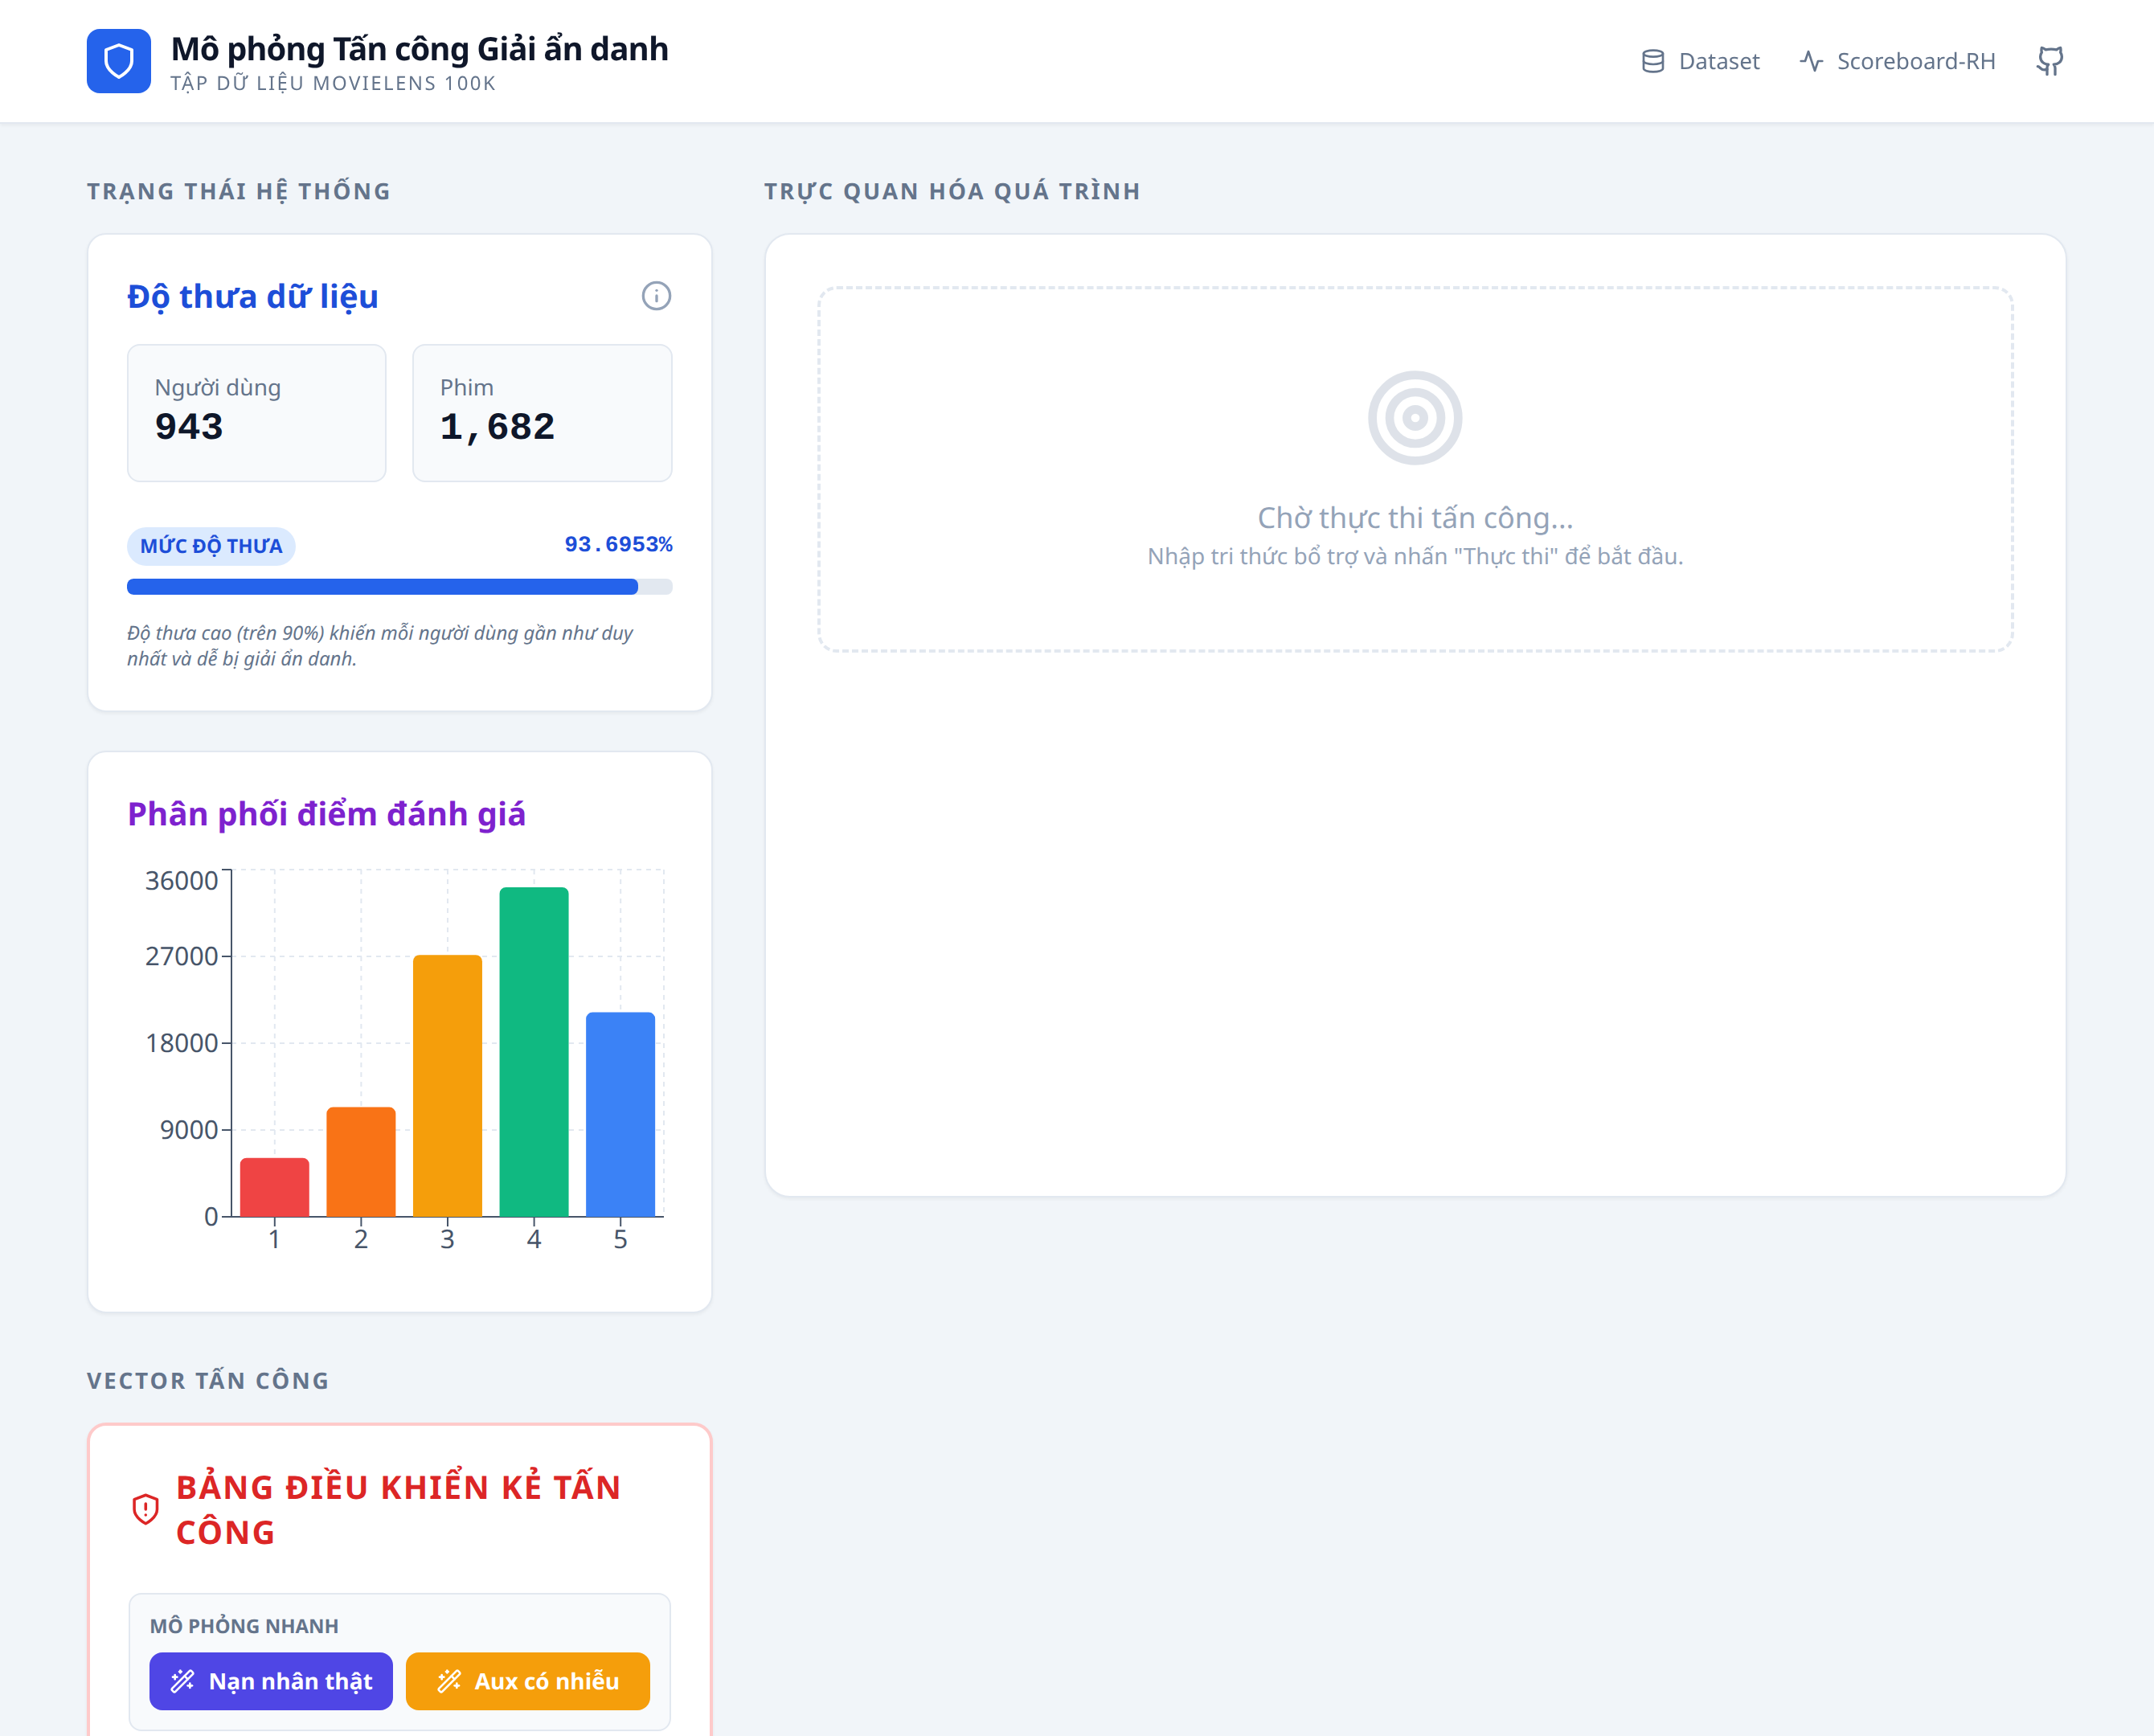
\includegraphics[width=0.95\linewidth]{figures/ui_01_overview.png}
\caption{Màn hình chính: thống kê độ thưa và bảng điều khiển kẻ tấn công}
\label{fig:ui_overview}
\end{figure}

\subsection{Nạp tri thức bổ trợ}
Chúng em dùng nút ``Nạn nhân thật'' để hệ thống lấy ngẫu nhiên dấu vân tay của một người dùng có thật. Hình~\ref{fig:ui_aux} cho thấy bốn phim được nạp vào bảng \textit{Thông tin đã biết}, mỗi phim kèm điểm, ngày, số người xem (support) và trọng số $wt(i)$. Có thể thấy các phim ít người xem (support nhỏ) được gán trọng số lớn hơn - đúng công thức~(\ref{eq:weight}).

\begin{figure}[!htb]
\centering
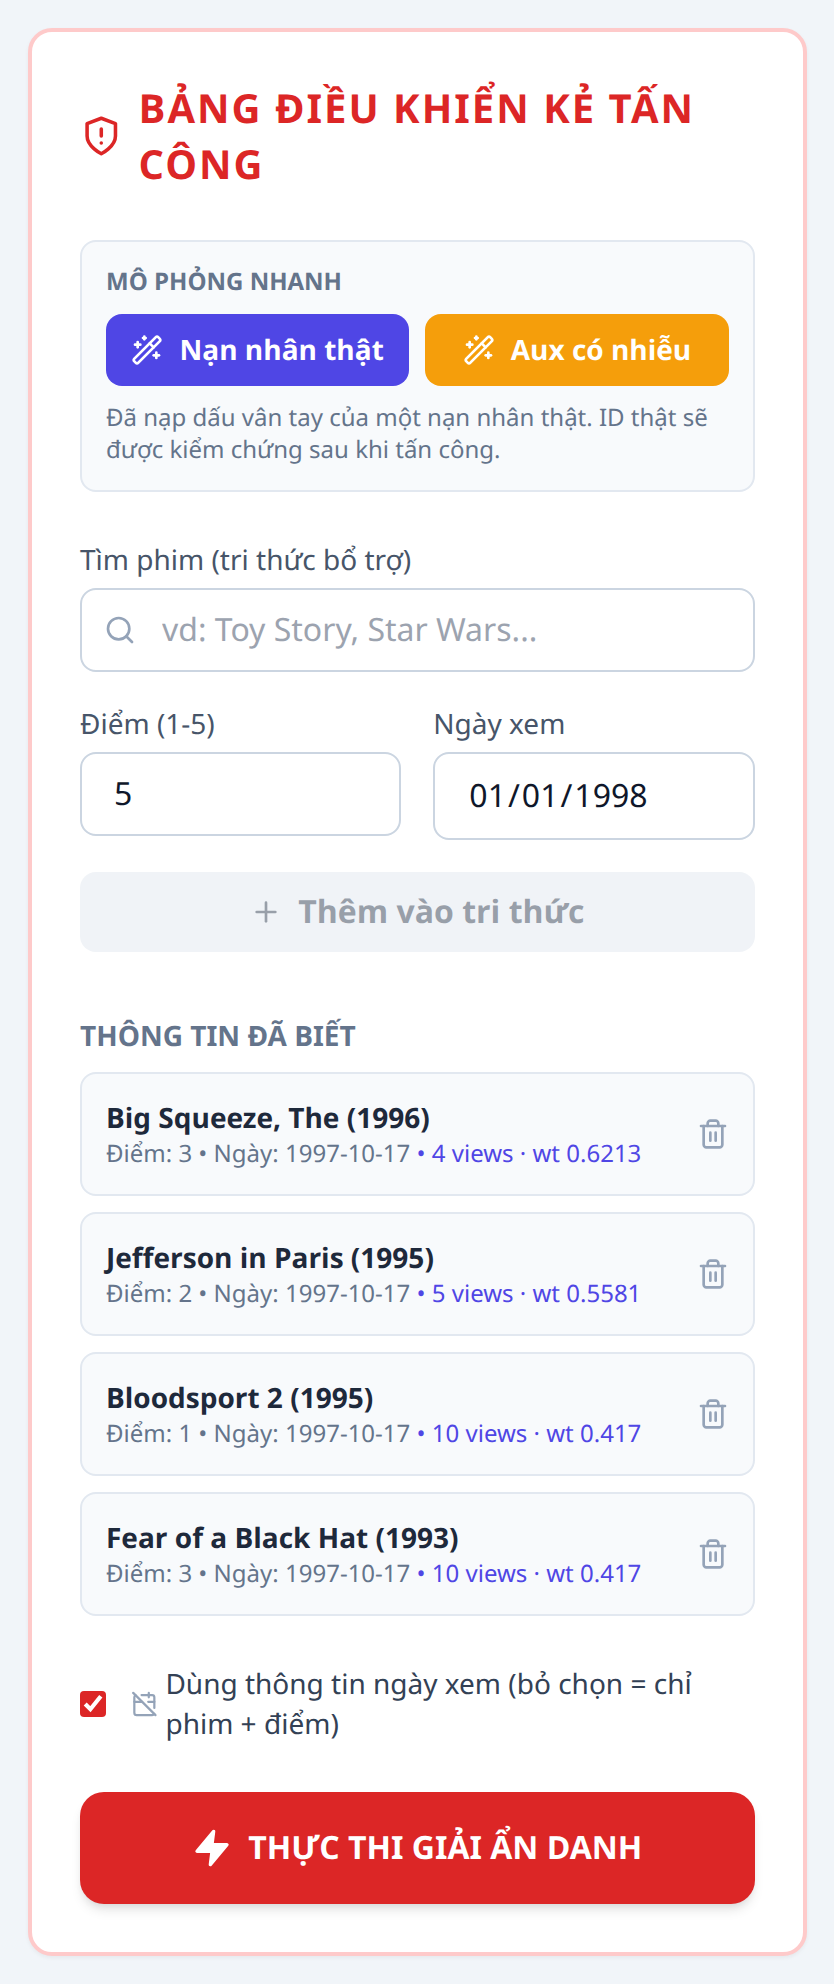
\includegraphics[width=0.46\linewidth]{figures/ui_02_aux_loaded.png}
\caption{Bảng điều khiển sau khi nạp aux: mỗi phim hiển thị support và trọng số độ hiếm}
\label{fig:ui_aux}
\end{figure}

\subsection{Kết quả định danh}
Sau khi nhấn ``Thực thi giải ẩn danh'', thuật toán xác định chính xác nạn nhân (Hình~\ref{fig:ui_result}): User \#373, eccentricity $3{,}8333$ (vượt xa ngưỡng $1{,}5$), độ tương tự $0{,}9886$. Đáng chú ý, không gian ứng viên chỉ còn 24 người - vì bốn phim hiếm trong aux đã thu hẹp đám đông xuống rất nhanh.

\begin{figure}[!htb]
\centering
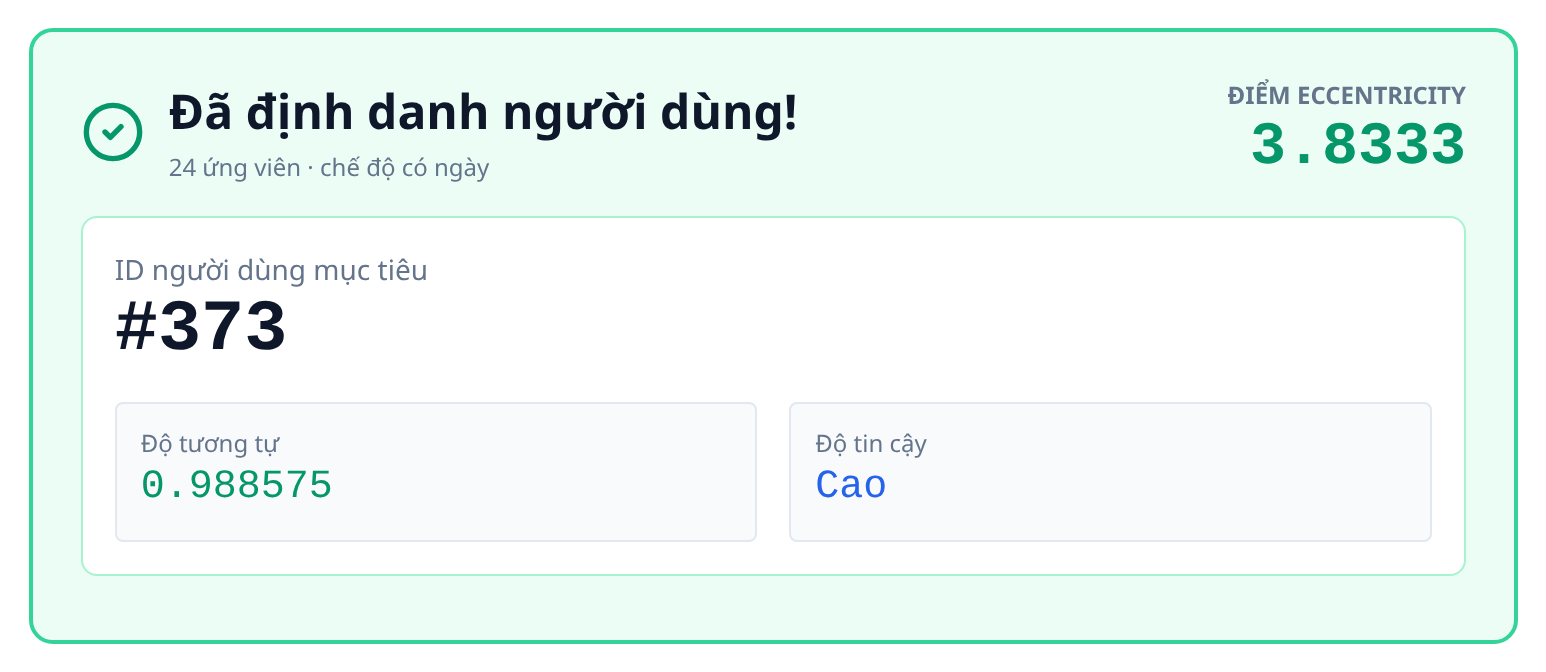
\includegraphics[width=0.95\linewidth]{figures/ui_03_result_identified.png}
\caption{Định danh thành công User \#373 với eccentricity $3{,}8333$}
\label{fig:ui_result}
\end{figure}

Quan trọng hơn, hệ thống phơi bày toàn bộ lịch sử xem phim của người này trong bảng \textit{Lịch sử riêng tư bị phơi bày} (Hình~\ref{fig:ui_history}) - 233 lượt đánh giá mà kẻ tấn công ban đầu hoàn toàn không biết. Đây chính là biểu hiện trực quan của ``rò rỉ riêng tư'': từ 4 mẩu thông tin, kẻ tấn công thu được toàn bộ chân dung hành vi của nạn nhân.

\begin{figure}[!htb]
\centering
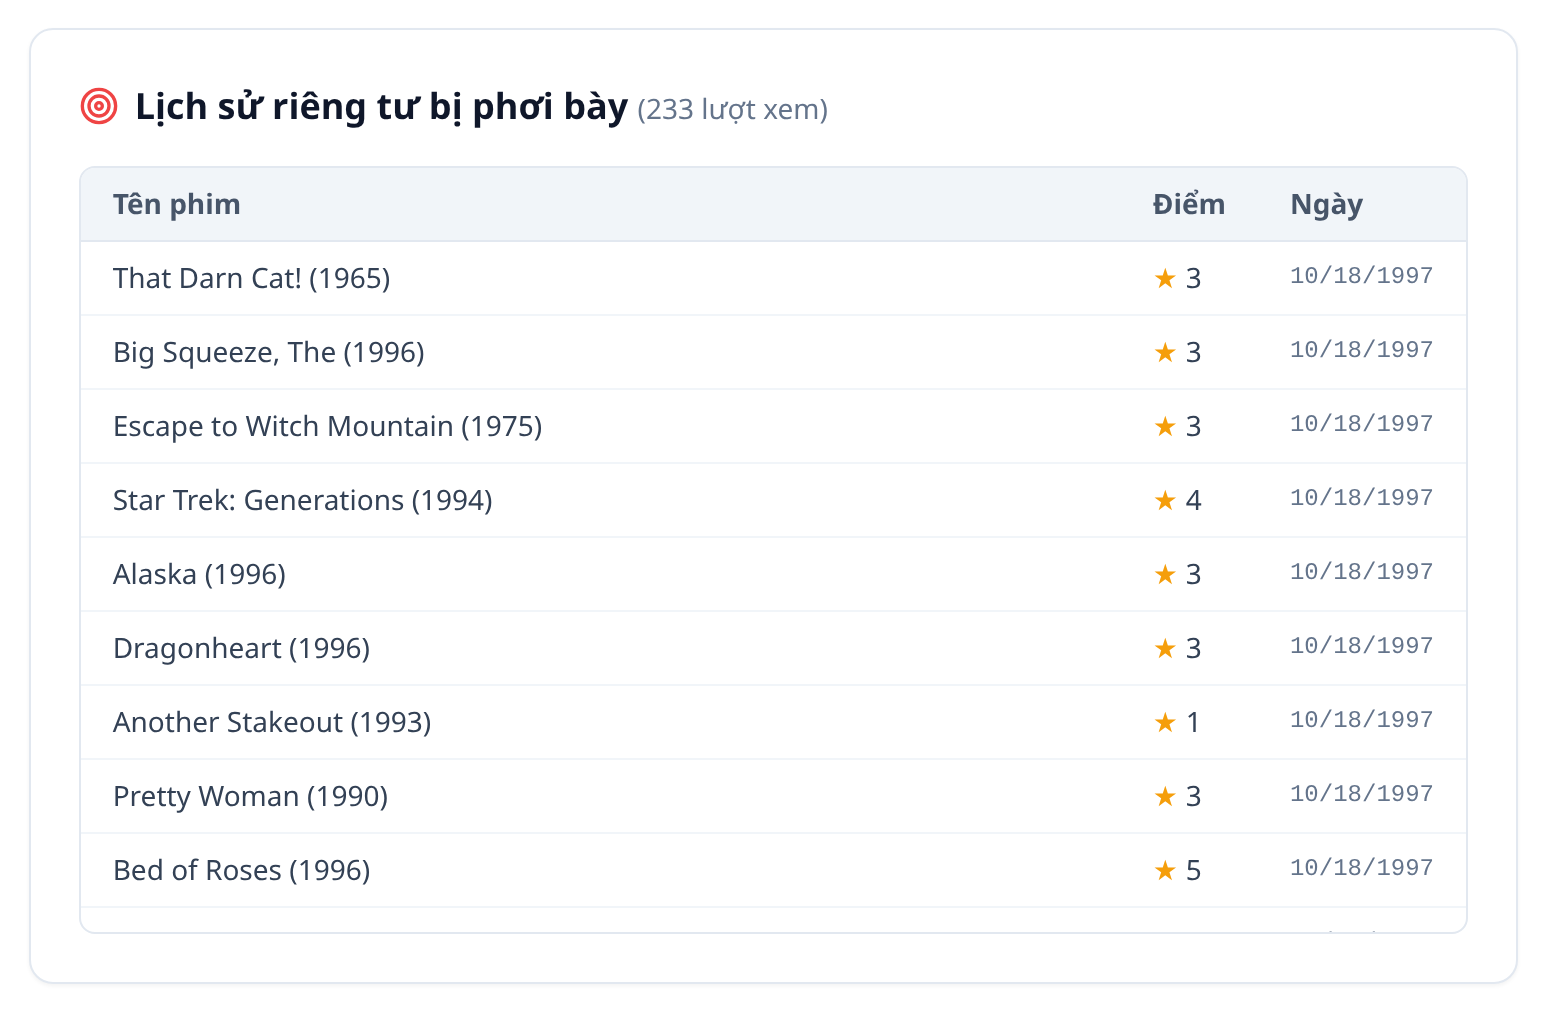
\includegraphics[width=0.82\linewidth]{figures/ui_04_exposed_history.png}
\caption{Lịch sử riêng tư của nạn nhân bị phơi bày hoàn toàn (233 lượt xem)}
\label{fig:ui_history}
\end{figure}

Hình~\ref{fig:ui_cand} là bảng xếp hạng \textit{Các ứng viên hàng đầu}: ứng viên hạng nhất (độ tương tự $\approx 0{,}99$) bỏ xa các ứng viên còn lại - minh họa trực quan ý nghĩa của eccentricity và lý do thuật toán tự tin kết luận.

\begin{figure}[!htb]
\centering
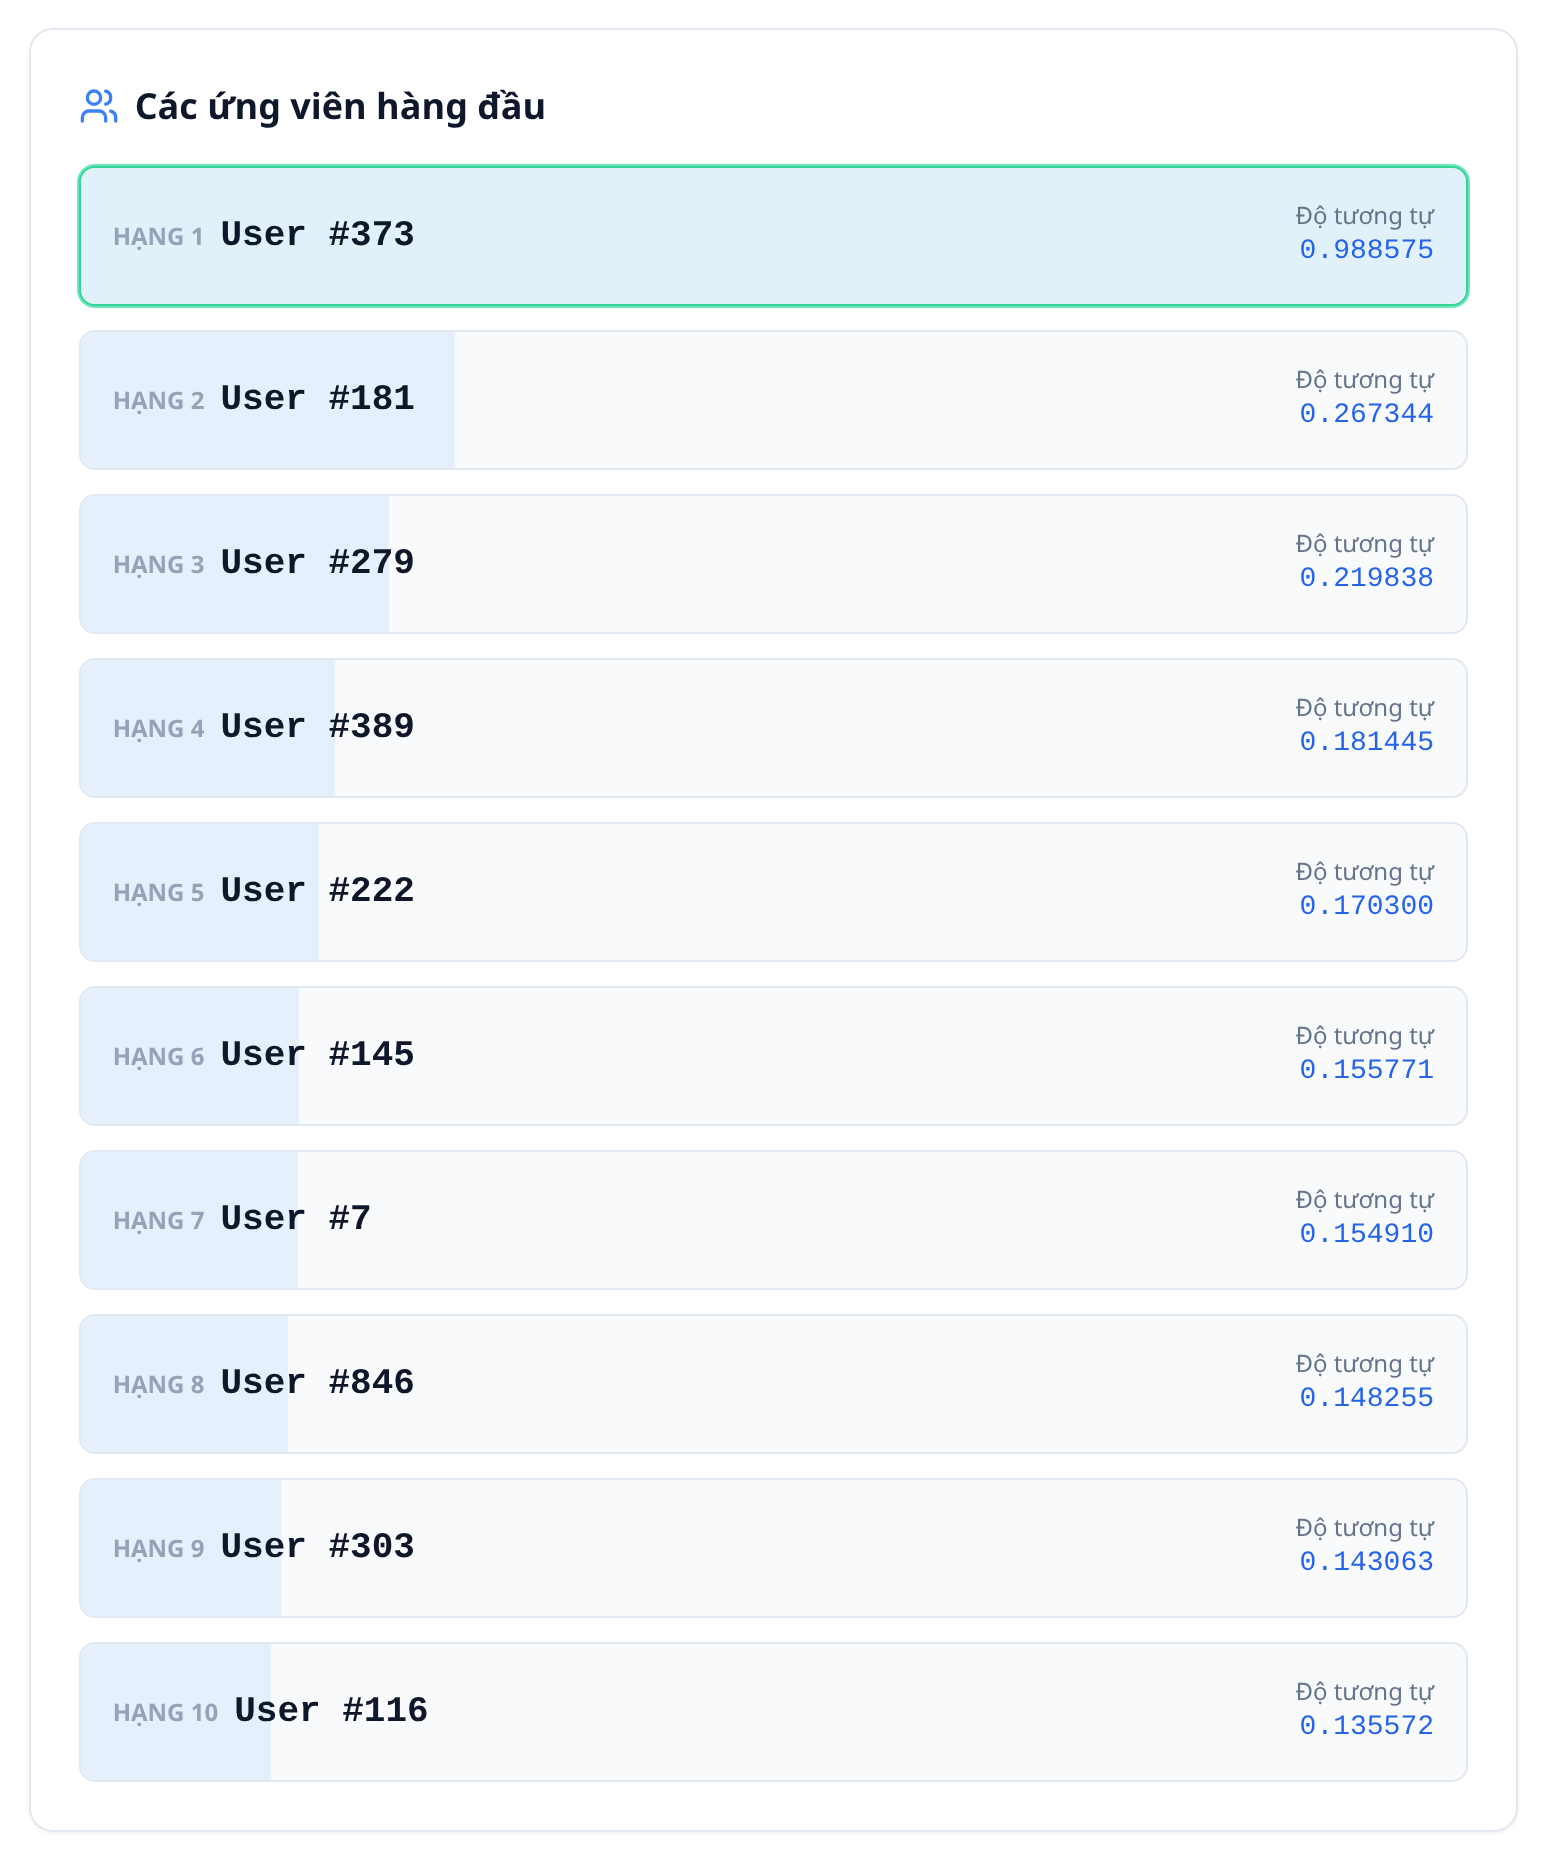
\includegraphics[width=0.80\linewidth]{figures/ui_06_top_candidates.png}
\caption{Bảng xếp hạng ứng viên: hạng nhất nổi bật hẳn so với phần còn lại}
\label{fig:ui_cand}
\end{figure}

\subsection{Tính bền vững trước thông tin nhiễu}
Để kiểm chứng tính bền vững, chúng em dùng nút ``Aux có nhiễu'': hệ thống lấy 6 phim của một nạn nhân thật nhưng cố ý làm sai điểm $\pm 1$ và sai ngày $\pm 14$ ngày. Dù vậy, thuật toán vẫn định danh đúng (Hình~\ref{fig:ui_noisy}): User \#278, eccentricity $5{,}1695$. Điều này xác nhận đặc tính ``robust'' cốt lõi: tấn công không đòi hỏi tri thức bổ trợ chính xác.

\begin{figure}[!htb]
\centering
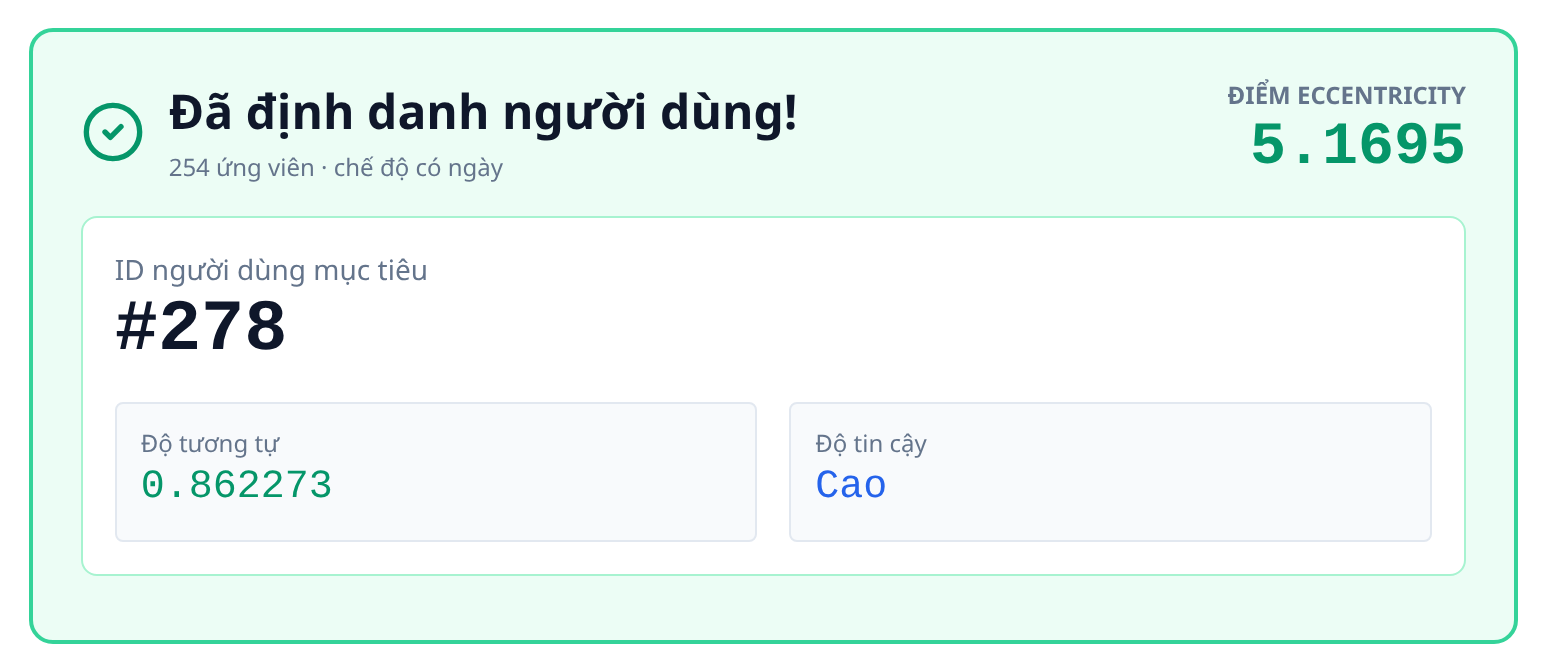
\includegraphics[width=0.95\linewidth]{figures/ui_05_robust_noisy.png}
\caption{Vẫn định danh đúng dù aux có nhiễu ($\pm 1$ điểm, $\pm 14$ ngày)}
\label{fig:ui_noisy}
\end{figure}

\section{Kiểm chứng trên dòng lệnh}

Để minh bạch, chúng em cũng chạy trực tiếp engine trên dòng lệnh. Hình~\ref{fig:term_demo} cho thấy một phiên tấn công vào nạn nhân thật \#200 với 6 phim chính xác: trong số 782 ứng viên, thuật toán chọn đúng người với độ tương tự tuyệt đối $1{,}0$, eccentricity $4{,}2504$, và phơi bày 216 lượt xem phim.

\begin{figure}[!htb]
\centering
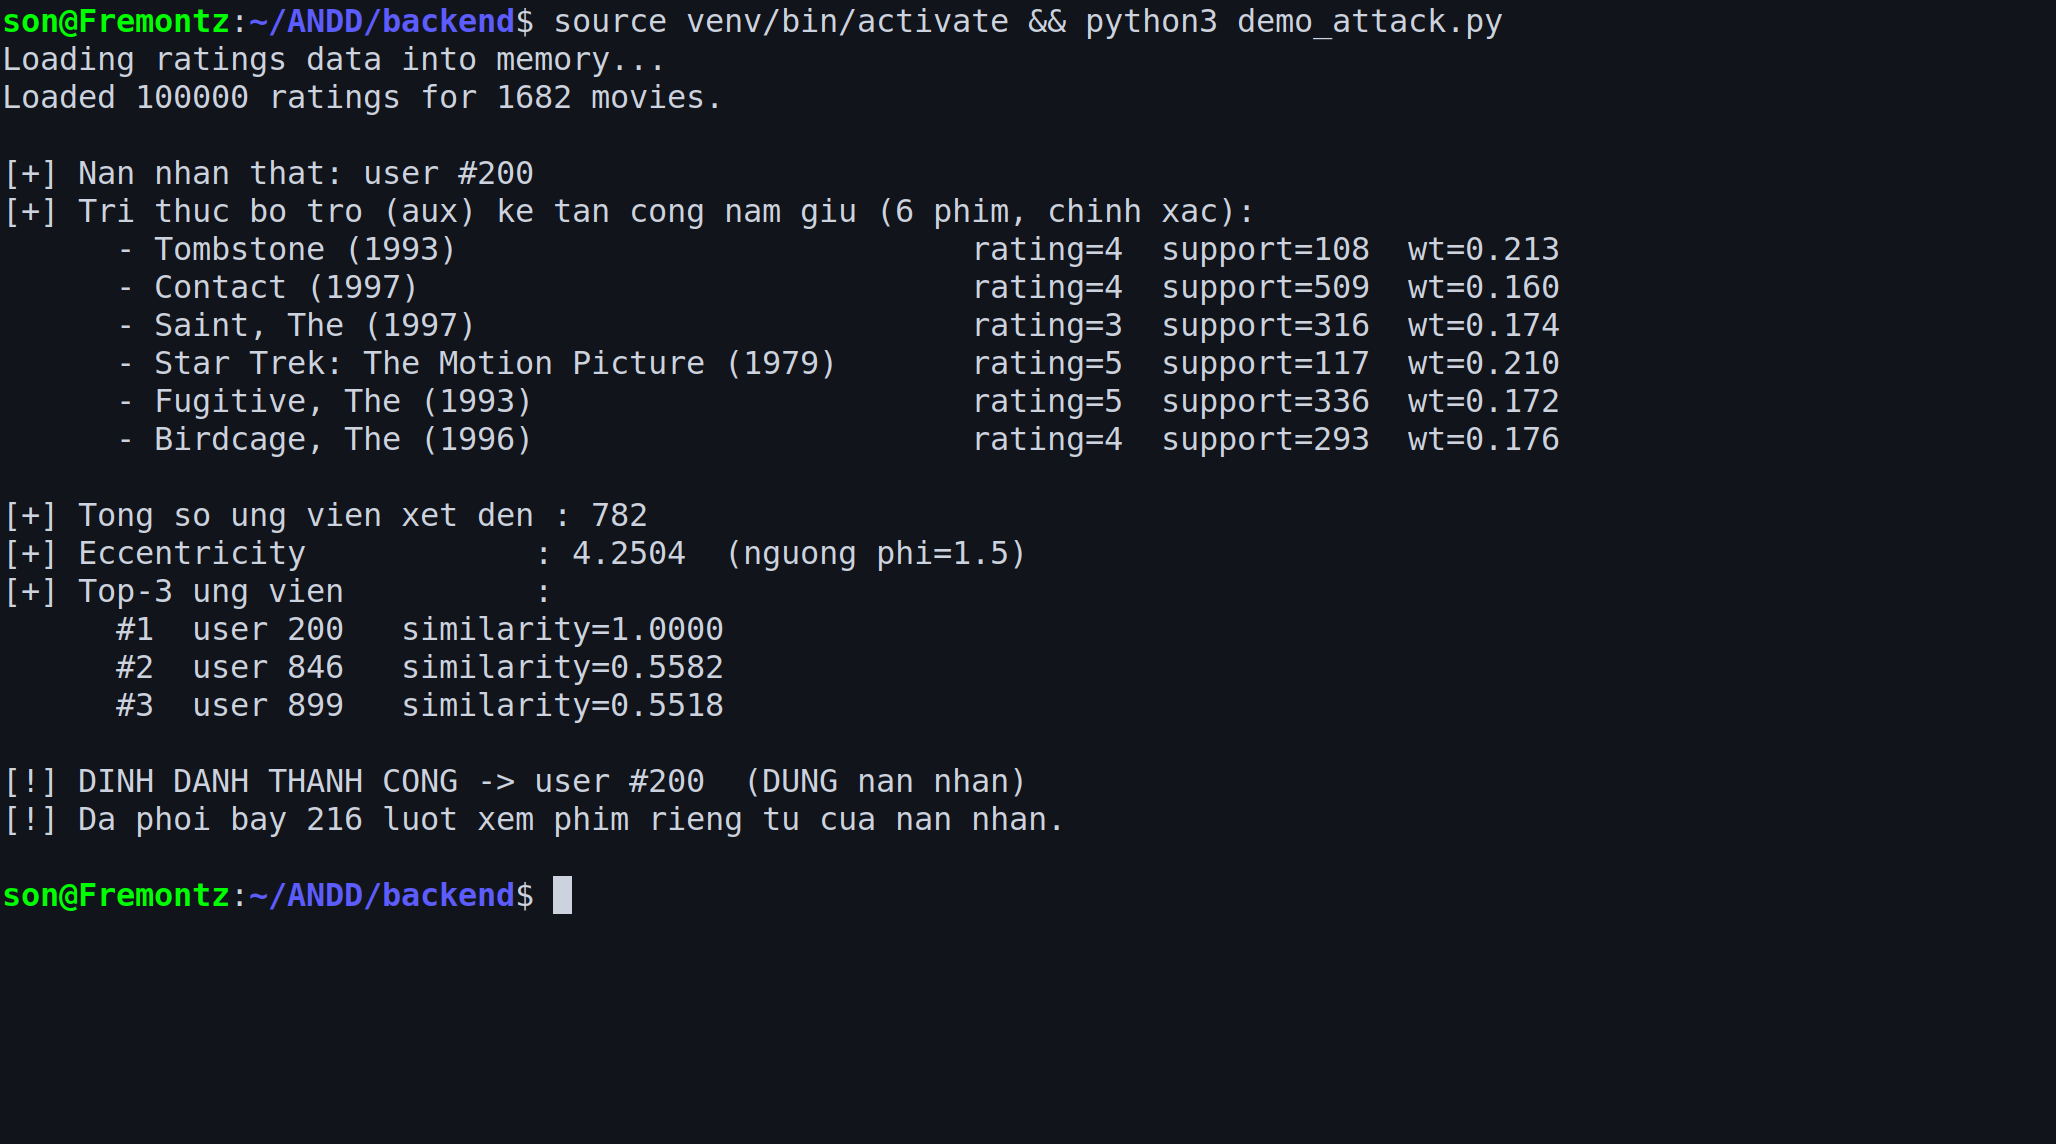
\includegraphics[width=0.92\linewidth]{figures/term_demo_attack.png}
\caption{Một phiên tấn công thật chạy trên dòng lệnh (nạn nhân \#200)}
\label{fig:term_demo}
\end{figure}

\section{Kết quả định lượng}

Phần này tái hiện kết quả chính của bài báo trên MovieLens. Chúng em chạy \texttt{experiment.py} trên 300 nạn nhân được chọn ngẫu nhiên (mỗi người đã xem $\ge 8$ phim), với năm mức số phim biết trước ($k \in \{2,3,4,6,8\}$) và bốn kịch bản. Kết quả thô in ở Hình~\ref{fig:term_exp} và tổng hợp ở Bảng~\ref{tab:results}.

\begin{figure}[!htb]
\centering
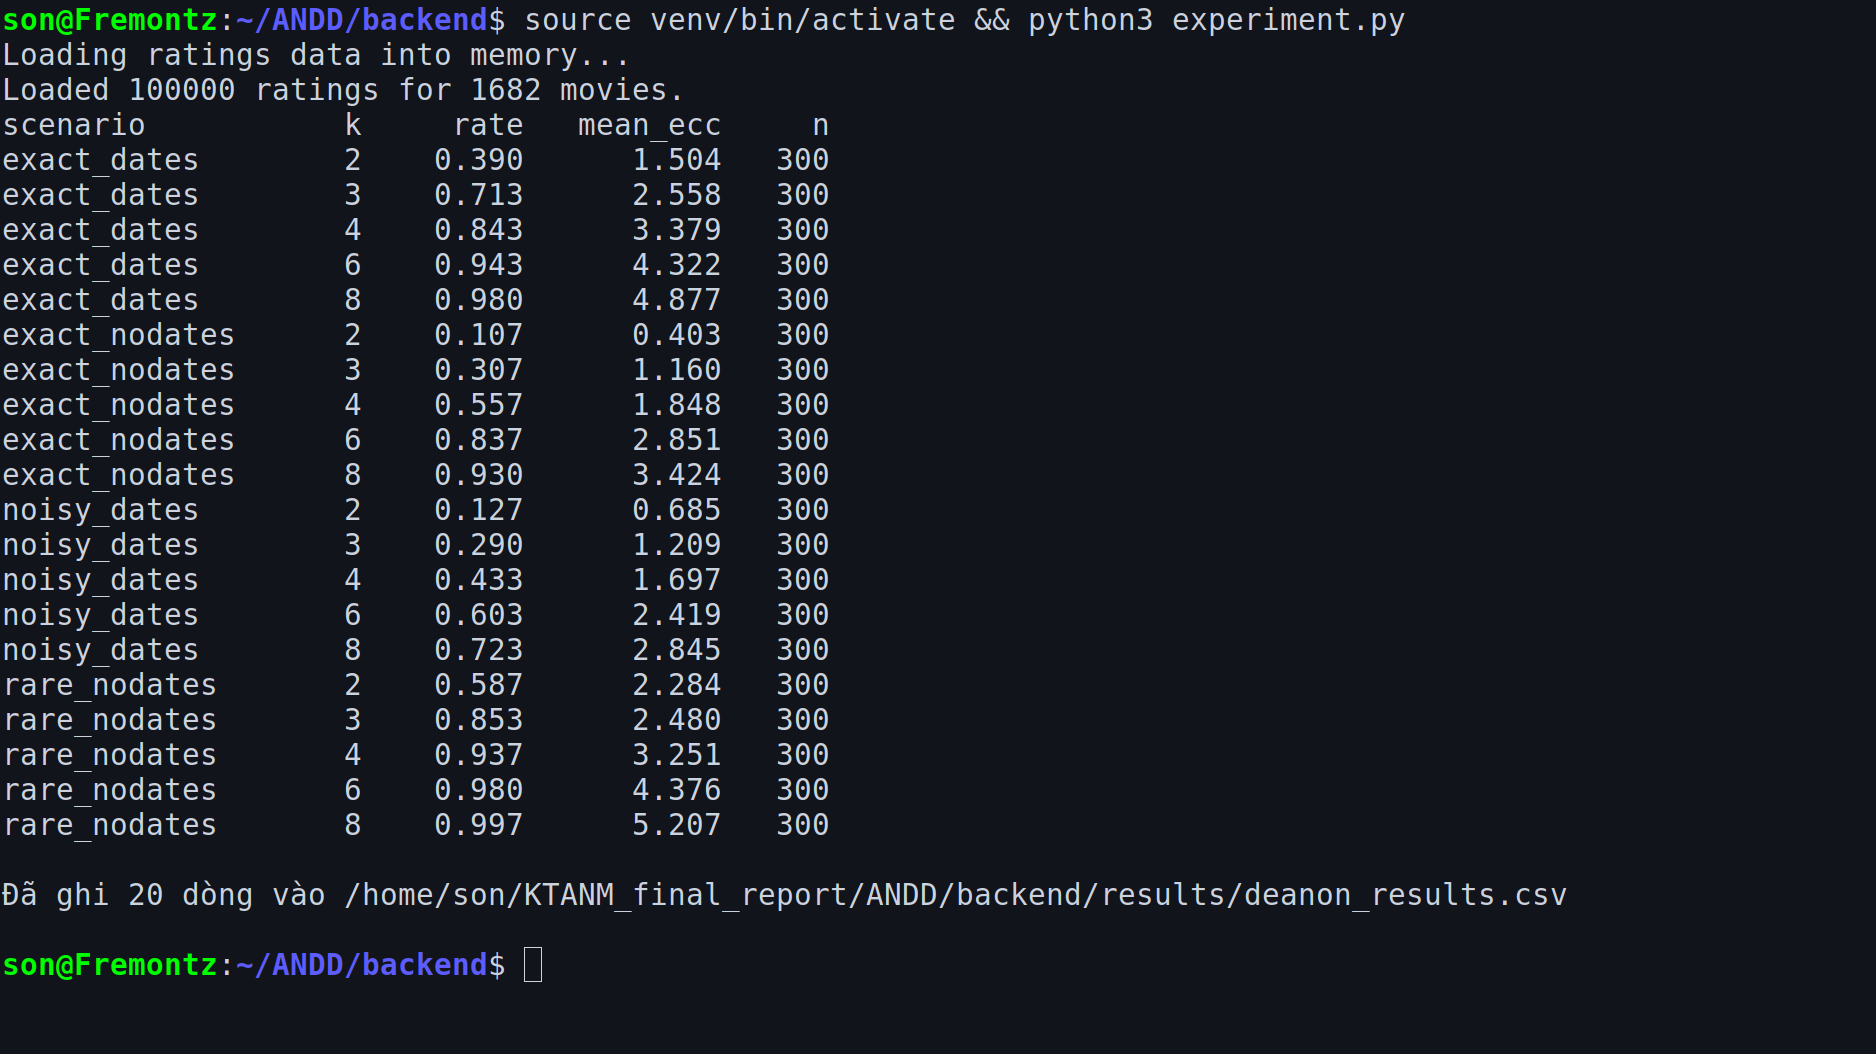
\includegraphics[width=0.82\linewidth]{figures/term_experiment.png}
\caption{Kết xuất (log) phiên chạy thực nghiệm trên 300 nạn nhân tại giao diện dòng lệnh, 4 kịch bản $\times$ 5 mức số phim}
\label{fig:term_exp}
\end{figure}

\begin{table}[!htb]
\centering
\caption{Tỉ lệ định danh đúng (\%) theo số phim biết trước và kịch bản}
\label{tab:results}
\renewcommand{\arraystretch}{1.3}
\begin{tabularx}{\linewidth}{X c c c c c}
\toprule
\textbf{Kịch bản} & \textbf{2 phim} & \textbf{3 phim} & \textbf{4 phim} & \textbf{6 phim} & \textbf{8 phim} \\
\midrule
Chính xác + có ngày        & 39{,}0 & 71{,}3 & 84{,}3 & 94{,}3 & \textbf{98{,}0} \\
Chính xác, không ngày      & 10{,}7 & 30{,}7 & 55{,}7 & 83{,}7 & 93{,}0 \\
Nhiễu ($\pm$1 điểm, $\pm$14 ngày) & 12{,}7 & 29{,}0 & 43{,}3 & 60{,}3 & 72{,}3 \\
Ưu tiên phim hiếm, không ngày & \textbf{58{,}7} & 85{,}3 & 93{,}7 & 98{,}0 & 99{,}7 \\
\bottomrule
\end{tabularx}
\end{table}

Hình~\ref{fig:chart_rate} và~\ref{fig:chart_ecc} trực quan hóa Bảng~\ref{tab:results} và eccentricity trung bình tương ứng.

\begin{figure}[!htb]
\centering
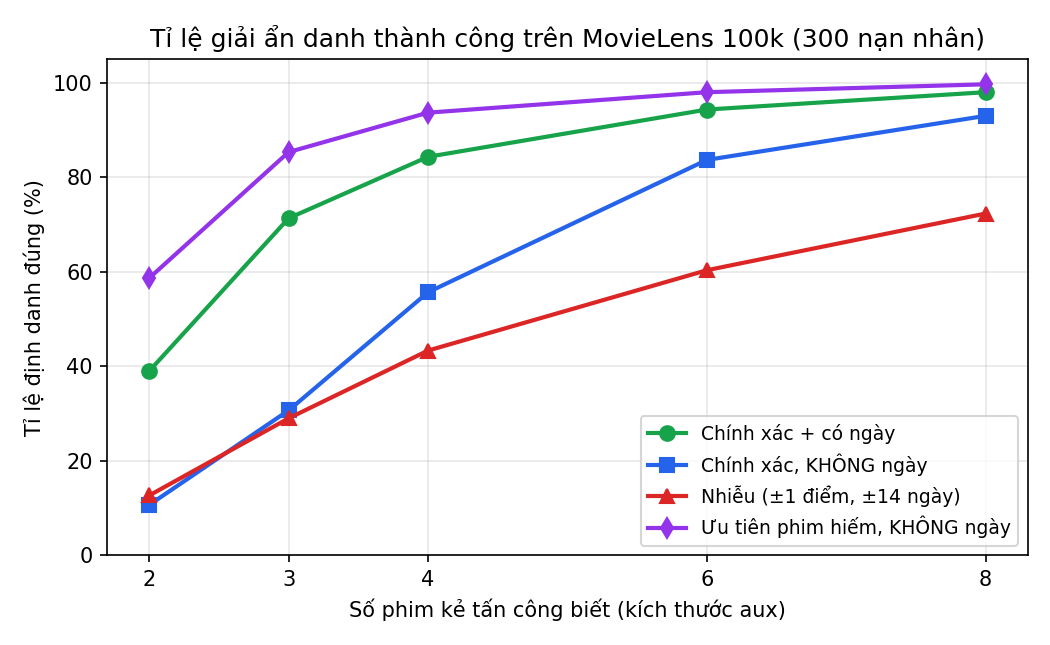
\includegraphics[width=0.85\linewidth]{figures/success_rate.png}
\caption{Tỉ lệ định danh thành công theo lượng tri thức bổ trợ}
\label{fig:chart_rate}
\end{figure}

\begin{figure}[!htb]
\centering
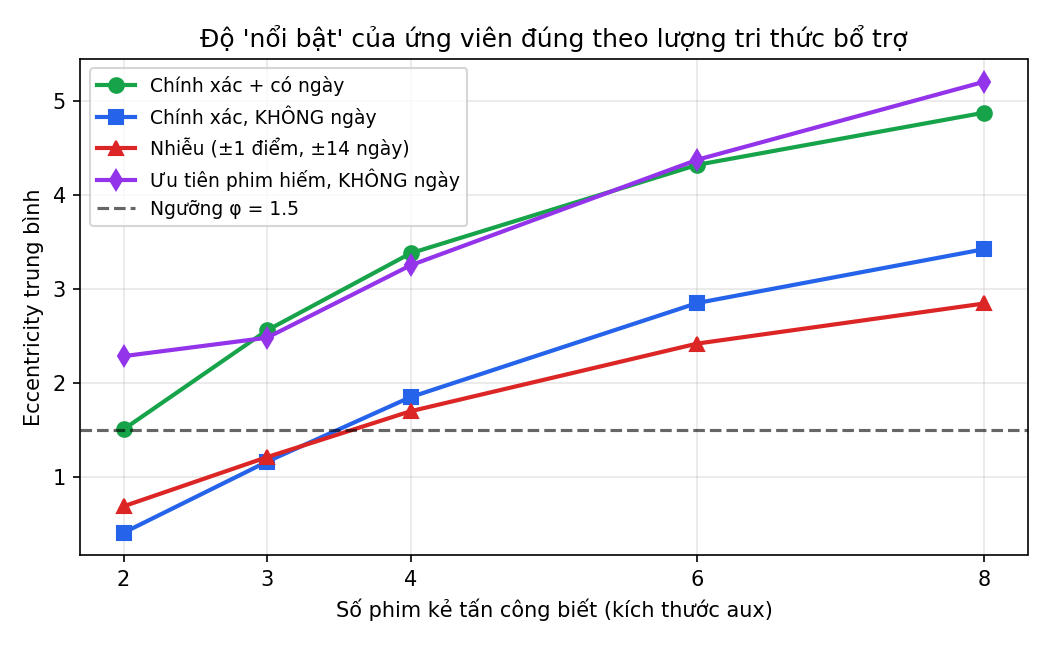
\includegraphics[width=0.85\linewidth]{figures/eccentricity.png}
\caption{Eccentricity trung bình theo lượng tri thức bổ trợ (đường nét đứt là ngưỡng $\phi=1{,}5$)}
\label{fig:chart_ecc}
\end{figure}

\section{Phân tích kết quả}

Các con số thật trên MovieLens tái hiện trung thực những kết luận của bài báo gốc:

\renewcommand{\labelitemi}{$-$}
\begin{itemize}
	\item \textbf{Càng nhiều tri thức, càng dễ định danh.} Với 8 phim chính xác kèm ngày, tỉ lệ định danh đúng đạt 98\% - rất gần con số 99\% mà bài báo công bố trên Netflix.
	\item \textbf{Ngày xem là thông tin giá trị nhưng không bắt buộc.} Bỏ thông tin ngày làm tỉ lệ giảm (ví dụ với 4 phim: từ $84{,}3\%$ xuống $55{,}7\%$), nhưng khi biết đủ 8 phim vẫn đạt $93\%$. Quyền riêng tư không được cứu vãn chỉ bằng cách giấu ngày.
	\item \textbf{Tấn công bền vững trước nhiễu.} Ngay cả khi điểm sai $\pm 1$ và ngày sai $\pm 14$ ngày, 8 phim vẫn cho $72{,}3\%$. Tri thức bổ trợ \textit{không cần chính xác}.
	\item \textbf{Phim hiếm là vũ khí mạnh nhất.} Khi ưu tiên phim ít người xem, chỉ 2 phim đã đủ định danh $58{,}7\%$ - cao hơn cả việc biết 4 phim phổ biến. Điều này khẳng định vai trò của trọng số độ hiếm $wt(i)$: một bộ phim nghệ thuật ít người biết tiết lộ nhiều hơn nhiều so với một bom tấn.
	\item \textbf{Eccentricity tăng đều theo lượng tri thức} (Hình~\ref{fig:chart_ecc}), cho thấy ứng viên đúng ngày càng ``nổi bật'' và cơ chế tự kiểm soát sai số hoạt động ổn định.
\end{itemize}

\section{Tình huống thất bại và ý nghĩa của ngưỡng}

Không phải mọi cuộc tấn công đều thành công - và đó là chủ ý thiết kế. Khi tri thức bổ trợ ít hoặc chỉ gồm phim phổ biến, nhiều người dùng có hồ sơ tương tự nhau, eccentricity tụt xuống dưới $1{,}5$ và thuật toán từ chối định danh thay vì đoán bừa. Trong một thực nghiệm với 5 phim phổ biến kèm nhiễu, ứng viên hạng nhất tuy đúng là nạn nhân nhưng eccentricity chỉ đạt $1{,}4995$ - sát ngưỡng - nên hệ thống vẫn báo ``không đủ tin cậy''. Cơ chế ngưỡng này giữ tỉ lệ dương tính giả ở mức thấp, khiến mỗi lần ``định danh thành công'' đều có độ tin cậy cao - đây chính là điều làm cho tấn công trở nên \textit{nguy hiểm} trên thực tế.

\newpage
\chapter{Thảo luận, phòng vệ và kết luận}
\label{chap:conclusion}

\section{Ý nghĩa về quyền riêng tư}

Thực nghiệm cho thấy một thông điệp rõ ràng: ẩn danh hóa không đồng nghĩa với riêng tư. Việc gỡ bỏ tên và số định danh khỏi một tập micro-data thưa gần như không bảo vệ được người dùng, vì chính tổ hợp hành vi của họ đã là một ``dấu vân tay'' duy nhất. Hệ quả còn nghiêm trọng hơn với đặc tính forward privacy: một khi một mẩu dữ liệu bị liên kết với danh tính thật, mọi liên kết về sau (kể cả với các định danh ảo mới) đều trở nên dễ dàng hơn. Trong bối cảnh thiết bị và ứng dụng di động liên tục thu thập dữ liệu vị trí, lịch sử duyệt web, danh sách ứng dụng đã cài - vốn cũng thưa và nhiều chiều - rủi ro giải ẩn danh là hoàn toàn hiện hữu.

\section{Các biện pháp phòng vệ}

\subsection{Vì sao k-anonymity không đủ}
Như đã phân tích ở Chương~\ref{chap:background}, k-anonymity giả định tách được quasi-identifier khỏi thuộc tính nhạy cảm - điều bất khả thi với dữ liệu hành vi, nơi mọi thuộc tính đều có thể là điểm liên kết. Trên dữ liệu nhiều chiều, để đạt $k$-ẩn danh phải khái quát hóa tới mức dữ liệu mất giá trị sử dụng.

\subsection{Riêng tư vi phân (Differential Privacy)}
Hướng phòng vệ vững chắc nhất hiện nay là riêng tư vi phân~\cite{dwork}: thay vì công bố micro-data, hệ thống chỉ trả lời các truy vấn tổng hợp và cố ý thêm nhiễu được hiệu chỉnh toán học, sao cho sự hiện diện hay vắng mặt của \textit{một} cá nhân gần như không ảnh hưởng tới kết quả. Cách này cung cấp bảo đảm riêng tư có thể chứng minh được, đánh đổi bằng một phần độ chính xác.

\subsection{Các biện pháp thực tiễn khác}
\renewcommand{\labelitemi}{$-$}
\begin{itemize}
	\item \textbf{Không công bố micro-data ở mức cá nhân}; chỉ phát hành thống kê tổng hợp đã thêm nhiễu.
	\item \textbf{Thêm nhiễu mạnh và lấy mẫu nhỏ:} tuy nhiên bài báo chứng minh nhiễu nhẹ là vô tác dụng - phải đủ mạnh tới mức ảnh hưởng giá trị sử dụng mới có hiệu quả.
	\item \textbf{Giảm chiều và gộp nhóm thuộc tính:} loại bỏ hoặc gộp các thuộc tính hiếm (vốn mang giá trị định danh cao nhất) trước khi công bố.
	\item \textbf{Kiểm soát truy cập và ràng buộc pháp lý:} hợp đồng sử dụng dữ liệu, cấm tái định danh, tối thiểu hóa dữ liệu thu thập ngay từ đầu.
\end{itemize}

\section{Hạn chế của nghiên cứu}

\renewcommand{\labelitemi}{$-$}
\begin{itemize}
	\item Tập MovieLens 100k nhỏ hơn nhiều so với Netflix (943 so với 500.000 người), nên đám đông ứng viên ít hơn và một số con số tuyệt đối lạc quan hơn thực tế; tuy nhiên các \textit{xu hướng} được tái hiện trung thực.
	\item Các tham số $\rho_0, d_0, \phi$ lấy theo bài báo, chưa tinh chỉnh riêng cho MovieLens.
	\item Hệ thống mô phỏng kịch bản kẻ tấn công đã biết bản ghi nạn nhân nằm trong tập công bố; chưa cài đặt đầy đủ biến thể phát hiện ``nạn nhân không có trong mẫu''.
\end{itemize}

\section{Kết luận}

Báo cáo đã nghiên cứu, mô phỏng và kiểm chứng bằng thực nghiệm thật lớp tấn công giải ẩn danh trên dữ liệu thưa của Narayanan-Shmatikov. Chúng em đã: (1) trình bày lại nền tảng lý thuyết và thuật toán Scoreboard-RH; (2) xây dựng, sửa lỗi và nâng cấp một ứng dụng web hoàn chỉnh - đặc biệt là sửa hàm cho điểm cho đúng công thức gốc, bổ sung chế độ không-ngày, phơi bày trọng số độ hiếm và mô-đun thực nghiệm; (3) tái hiện thành công các kết quả chính của bài báo trên MovieLens 100k, với 8 phim cho tỉ lệ định danh đúng tới 98\%, và chứng minh tính bền vững trước nhiễu cũng như sức mạnh đặc biệt của các thuộc tính hiếm.

Kết quả khẳng định một bài học nền tảng của an toàn dữ liệu hiện đại: trong thế giới dữ liệu thưa và nhiều chiều, riêng tư phải được bảo đảm bằng các cơ chế có cơ sở toán học như riêng tư vi phân, chứ không thể trông cậy vào việc ``gỡ bỏ thông tin định danh''.

\newpage

\renewcommand{\bibname}{Tài liệu tham khảo}
\clearpage
\phantomsection
\addcontentsline{toc}{chapter}{{TÀI LIỆU THAM KHẢO}}

\begin{thebibliography}{[99]}
\fontsize{13}{16}\selectfont

\bibitem{narayanan} A. Narayanan, V. Shmatikov, ``Robust De-anonymization of Large Sparse Datasets,'' \textit{Proc. IEEE Symposium on Security and Privacy (S\&P)}, pp.~111-125, 2008. DOI: \url{https://doi.org/10.1109/SP.2008.33}

\bibitem{netflix} J. Bennett, S. Lanning, ``The Netflix Prize,'' \textit{Proc. KDD Cup and Workshop}, 2007. [Online]. Available: \url{https://web.archive.org/web/20090924184639/http://www.netflixprize.com/}

\bibitem{movielens} F. M. Harper, J. A. Konstan, ``The MovieLens Datasets: History and Context,'' \textit{ACM Transactions on Interactive Intelligent Systems (TiiS)}, vol.~5, no.~4, art.~19, 2015. DOI: \url{https://doi.org/10.1145/2827872}

\bibitem{sweeney} L. Sweeney, ``k-anonymity: A Model for Protecting Privacy,'' \textit{International Journal of Uncertainty, Fuzziness and Knowledge-Based Systems}, vol.~10, no.~5, pp.~557-570, 2002. DOI: \url{https://doi.org/10.1142/S0218488502001648}

\bibitem{ldiversity} A. Machanavajjhala, J. Gehrke, D. Kifer, M. Venkitasubramaniam, ``l-diversity: Privacy Beyond k-anonymity,'' \textit{Proc. IEEE ICDE}, 2006. DOI: \url{https://doi.org/10.1109/ICDE.2006.1}

\bibitem{tcloseness} N. Li, T. Li, S. Venkatasubramanian, ``t-Closeness: Privacy Beyond k-Anonymity and l-Diversity,'' \textit{Proc. IEEE ICDE}, pp.~106-115, 2007. DOI: \url{https://doi.org/10.1109/ICDE.2007.367856}

\bibitem{aol} M. Barbaro, T. Zeller, ``A Face Is Exposed for AOL Searcher No.~4417749,'' \textit{The New York Times}, Aug.~2006. [Online]. Available: \url{https://www.nytimes.com/2006/08/09/technology/09aol.html}

\bibitem{demontjoye} Y.-A. de Montjoye, C. A. Hidalgo, M. Verleysen, V. D. Blondel, ``Unique in the Crowd: The Privacy Bounds of Human Mobility,'' \textit{Scientific Reports}, vol.~3, art.~1376, 2013. DOI: \url{https://doi.org/10.1038/srep01376}

\bibitem{demontjoye2} Y.-A. de Montjoye, L. Radaelli, V. K. Singh, A. ``Sandy'' Pentland, ``Unique in the Shopping Mall: On the Reidentifiability of Credit Card Metadata,'' \textit{Science}, vol.~347, no.~6221, pp.~536-539, 2015. DOI: \url{https://doi.org/10.1126/science.1256297}

\bibitem{vppa} Electronic Privacy Information Center, ``The Video Privacy Protection Act (VPPA).'' [Online]. Available: \url{https://epic.org/privacy/vppa/}

\bibitem{frankowski} D. Frankowski, D. Cosley, S. Sen, L. Terveen, J. Riedl, ``You Are What You Say: Privacy Risks of Public Mentions,'' \textit{Proc. ACM SIGIR}, pp.~565-572, 2006. DOI: \url{https://doi.org/10.1145/1148170.1148267}

\bibitem{dwork} C. Dwork, ``Differential Privacy,'' \textit{Proc. ICALP 2006}, LNCS 4052, pp.~1-12, 2006. DOI: \url{https://doi.org/10.1007/11787006_1}

\bibitem{netflixsuit} R. Singel, ``Netflix Spilled Your Brokeback Mountain Secret, Lawsuit Claims,'' \textit{Wired}, Dec.~2009. [Online]. Available: \url{https://www.wired.com/2009/12/netflix-privacy-lawsuit/}

\bibitem{fastapi} S. Ram\'irez, ``FastAPI - Modern, Fast Web Framework for Building APIs with Python.'' [Online]. Available: \url{https://fastapi.tiangolo.com/}

\bibitem{react} Meta Open Source, ``React - The Library for Web and Native User Interfaces.'' [Online]. Available: \url{https://react.dev/}

\end{thebibliography}

\newpage
\clearpage
\phantomsection

\addcontentsline{toc}{chapter}{{PHỤ LỤC}}
\chapter*{Phụ lục}
\setcounter{table}{0}
\renewcommand{\thetable}{A.\arabic{table}}

\section*{A. Hướng dẫn cài đặt và chạy demo}

Mã nguồn dự án gồm hai phần: \texttt{backend/} (FastAPI + engine tấn công) và \texttt{frontend/} (React + Vite). Các bước chạy:

\vspace{0.3cm}
\noindent\textbf{Backend (cổng 8000):}
\begin{lstlisting}[language=bash]
cd backend
python3 -m venv venv && source venv/bin/activate
pip install -r requirements.txt
python data_loader.py          # nap MovieLens 100k vao SQLite (chi lan dau)
uvicorn main:app --reload      # chay API tai http://localhost:8000
\end{lstlisting}

\noindent\textbf{Frontend (cổng 5173):}
\begin{lstlisting}[language=bash]
cd frontend
npm install
npm run dev                    # mo http://localhost:5173
\end{lstlisting}

\noindent\textbf{Chạy thực nghiệm định lượng và vẽ biểu đồ:}
\begin{lstlisting}[language=bash]
cd backend && source venv/bin/activate
python experiment.py           # sinh results/deanon_results.csv
python plot_results.py         # sinh success_rate.png, eccentricity.png
python demo_attack.py          # mot phien tan cong mau tren dong lenh
\end{lstlisting}

\section*{B. Mã nguồn các thành phần chính}
Phần này in mã nguồn đầy đủ của các thành phần cốt lõi, được tham chiếu trực tiếp từ Chương~\ref{chap:impl}.

\setcounter{lstlisting}{0}
\renewcommand{\thelstlisting}{A.\arabic{lstlisting}}
\lstset{basicstyle=\ttfamily\fontsize{8}{9.5}\selectfont}

\lstinputlisting[language=Python, caption={\texttt{attack\_engine.py} - engine cài đặt thuật toán Scoreboard-RH, gồm hàm cho điểm, eccentricity và \texttt{sample\_aux\_from\_user}}, label={lst:engine}]{_scripts/attack_engine.py}

\lstinputlisting[language=Python, caption={\texttt{main.py} - REST API FastAPI phơi bày các endpoint tấn công}, label={lst:api}]{_scripts/main.py}

\lstinputlisting[language=Python, caption={\texttt{experiment.py} - thực nghiệm định lượng tỉ lệ định danh trên 300 nạn nhân}, label={lst:experiment}]{_scripts/experiment.py}

\lstinputlisting[language=Python, caption={\texttt{demo\_attack.py} - một phiên tấn công mẫu chạy trên dòng lệnh}, label={lst:demo}]{_scripts/demo_attack.py}


\end{document}
